%%
%% Automatically generated file from DocOnce source
%% (https://github.com/hplgit/doconce/)
%%

% #define PREAMBLE

% #ifdef PREAMBLE
%-------------------- begin preamble ----------------------

% Style: T4 (Springer)
% Use svmono.cls with doconce modifications for bibliography (svmonodo.cls)
\documentclass[graybox,sectrefs,envcountresetchap,open=right,final]{svmonodo}

% Use t4.sty with doconce modifications (t4do.sty)
\usepackage{t4do}
\special{papersize=178mm,254mm}

\listfiles               %  print all files needed to compile this document

\usepackage{relsize,makeidx,color,setspace,amsmath,amsfonts,amssymb}
\usepackage[table]{xcolor}
\usepackage{bm,ltablex,microtype}

\usepackage{graphicx}

% Packages for typesetting blocks of computer code
\usepackage{fancyvrb,framed,moreverb}

% Define colors
\definecolor{orange}{cmyk}{0,0.4,0.8,0.2}
\definecolor{tucorange}{rgb}{1.0,0.64,0}
\definecolor{darkorange}{rgb}{.71,0.21,0.01}
\definecolor{darkgreen}{rgb}{.12,.54,.11}
\definecolor{myteal}{rgb}{.26, .44, .56}
\definecolor{gray}{gray}{0.45}
\definecolor{mediumgray}{gray}{.8}
\definecolor{lightgray}{gray}{.95}
\definecolor{brown}{rgb}{0.54,0.27,0.07}
\definecolor{purple}{rgb}{0.5,0.0,0.5}
\definecolor{darkgray}{gray}{0.25}
\definecolor{darkblue}{rgb}{0,0.08,0.45}
\definecolor{darkblue2}{rgb}{0,0,0.8}
\definecolor{lightred}{rgb}{1.0,0.39,0.28}
\definecolor{lightgreen}{rgb}{0.48,0.99,0.0}
\definecolor{lightblue}{rgb}{0.53,0.81,0.92}
\definecolor{lightblue2}{rgb}{0.3,0.3,1.0}
\definecolor{lightpurple}{rgb}{0.87,0.63,0.87}
\definecolor{lightcyan}{rgb}{0.5,1.0,0.83}

\colorlet{comment_green}{green!50!black}
\colorlet{string_red}{red!60!black}
\colorlet{keyword_pink}{magenta!70!black}
\colorlet{indendifier_green}{green!70!white}

% Backgrounds for code
\definecolor{cbg_gray}{rgb}{.95, .95, .95}
\definecolor{bar_gray}{rgb}{.92, .92, .92}

\definecolor{cbg_yellowgray}{rgb}{.95, .95, .85}
\definecolor{bar_yellowgray}{rgb}{.95, .95, .65}

\colorlet{cbg_yellow2}{yellow!10}
\colorlet{bar_yellow2}{yellow!20}

\definecolor{cbg_yellow1}{rgb}{.98, .98, 0.8}
\definecolor{bar_yellow1}{rgb}{.98, .98, 0.4}

\definecolor{cbg_red1}{rgb}{1, 0.85, 0.85}
\definecolor{bar_red1}{rgb}{1, 0.75, 0.85}

\definecolor{cbg_blue1}{rgb}{0.988235,0.964706,0.862745}
\definecolor{bar_blue1}{rgb}{0.988235,0.964706,0.862745}

\usepackage{listingsutf8}

% Common lstlisting parameters

\usepackage{calc}
\newlength{\lstboxwidth}  % width of lst box
\newlength{\framethickness}
\setlength{\framethickness}{0.5mm}
% for frame=trbl and a framerule that has significant size, set
% xleftmargin=5mm and xrightmargin=5mm.

\lstset{
  basicstyle=\small \ttfamily,
  breaklines=false,          % break/wrap lines
  breakatwhitespace=true,    % let linebreaks happen at whitespace
  breakindent=40pt,
  tab=,
  tabsize=4,                 % tab means 4 spaces
  %belowskip=\smallskipamount,  % space between code and text below
  xleftmargin=2mm,           % indentation of code frame
  xrightmargin=0mm,
  framexleftmargin=2mm,      % add frame space to the left of the code box
  %numbers=left,             % put line numbers on the left
  %stepnumber=2,             % stepnumber=1 numbers each line, =n every n lines
  framerule=\framethickness, % thickness of frame
  aboveskip=2ex,             % vertical space above code frame
  showstringspaces=false,    % show spaces in strings with an underscore
  showspaces=false,          % show spaces with an underscore
  showtabs=false,
  keepspaces=true,
  columns=fullflexible,      % tighter character kerning, like verb
  escapeinside={(*@}{@*)},   % (*@ \pause @*) in slides and math in code blocks
  extendedchars=\true,       % allows non-ascii chars, does not work with utf-8
}

% Internally defined styles for lstlisting

% Use this one without additional background color
\lstdefinestyle{blue1}{              % blue1 background for code snippets
backgroundcolor=\color{cbg_blue1},
}

% Use this one without additional background color
% (same as blue1, but with bar_blue1 frame)
\lstdefinestyle{blue1bar}{           % blue1 background for complete programs
backgroundcolor=\color{cbg_blue1},
frame=tb,                            % include frame
rulecolor=\color{bar_blue1},         % frame color
}

% Use this one without additional background color
\lstdefinestyle{gray}{
backgroundcolor=\color{cbg_gray},
%frame=tb,                            % include frame
%framerule=0.4pt                      % thickness of frame
rulecolor=\color{black!40},           % frame color
}

\lstdefinestyle{simple}{
commentstyle={},
}

% end of custom lstdefinestyles

\usepackage[T1]{fontenc}
%\usepackage[latin1]{inputenc}
\usepackage{ucs}
\usepackage[utf8x]{inputenc}

\usepackage{lmodern}         % Latin Modern fonts derived from Computer Modern

% Hyperlinks in PDF:

\usepackage{hyperref}
\hypersetup{
    breaklinks=true,
    colorlinks=true,
    linkcolor=black,
    urlcolor=black,
    citecolor=black,
    filecolor=black,
    %filecolor=blue,
    pdfmenubar=true,
    pdftoolbar=true,
    bookmarksdepth=3   % Uncomment (and tweak) for PDF bookmarks with more levels than the TOC
    }
%\hyperbaseurl{}   % hyperlinks are relative to this root

\setcounter{tocdepth}{3}  % levels in table of contents

% Must use \VerbatimFootnotes since there are footnotes with inline
% verbatim text, but \VerbatimFootnotes interfers
%with svmonodo/t2do/t4do styles so that the footmisc package settings
% do not work and the typesetting looks strange...
%\VerbatimFootnotes must come after hyperref and footmisc packages
\VerbatimFootnotes

% Tricks for having figures close to where they are defined:
% 1. define less restrictive rules for where to put figures
\setcounter{topnumber}{2}
\setcounter{bottomnumber}{2}
\setcounter{totalnumber}{4}
\renewcommand{\topfraction}{0.95}
\renewcommand{\bottomfraction}{0.95}
\renewcommand{\textfraction}{0}
\renewcommand{\floatpagefraction}{0.75}
% floatpagefraction must always be less than topfraction!
% 2. ensure all figures are flushed before next section
\usepackage[section]{placeins}
% 3. enable begin{figure}[H] (often leads to ugly pagebreaks)
%\usepackage{float}\restylefloat{figure}

\usepackage{wrapfig,calc}
\usepackage[framemethod=TikZ]{mdframed}  % use latest version: https://github.com/marcodaniel/mdframed

% --- begin definitions of admonition environments ---

% Admonition style "graybox2" is a gray or colored box with a square
% frame, except for the summary admon which has horizontal rules only
% Note: this admonition type cannot handle verbatim text!
\colorlet{graybox2_warning_background}{darkgreen!40!white}

% colored box of 80% width
\newcommand{\grayboxhrules}[1]{\begin{center}
\colorbox{graybox2_warning_background}{\rule{6pt}{0pt}
\begin{minipage}{0.8\linewidth}
\parbox[t]{0mm}{\rule[0pt]{0mm}{0.5\baselineskip}}\hrule
\vspace*{0.5\baselineskip}\noindent #1
\parbox[t]{0mm}{\rule[-0.5\baselineskip]{0mm}%
{\baselineskip}}\hrule\vspace*{0.5\baselineskip}\end{minipage}
\rule{6pt}{0pt}}\end{center}}

% Fallback for verbatim content in \grayboxhrules
\newmdenv[
  backgroundcolor=graybox2_warning_background,
  skipabove=15pt,
  skipbelow=15pt,
  leftmargin=23,
  rightmargin=23,
  needspace=0pt,
]{graybox2mdframed}

\newenvironment{graybox2admon}[1][]{
\begin{graybox2mdframed}[frametitle=#1]
}
{
\end{graybox2mdframed}
}

% --- end of definitions of admonition environments ---

% prevent orhpans and widows
\clubpenalty = 10000
\widowpenalty = 10000

\newenvironment{doconceexercise}{}{}
\newcounter{doconceexercisecounter}
% --- begin definition of \listofexercises command ---
\makeatletter
\newcommand\listofexercises{
\chapter*{List of Exercises
          \@mkboth{List of Exercises}{List of Exercises}}
\markboth{List of Exercises}{List of Exercises}
\@starttoc{loe}
}
\newcommand*{\l@doconceexercise}{\@dottedtocline{0}{0pt}{6.5em}}
\makeatother
% --- end definition of \listofexercises command ---


% Let exercises, problems, and projects be numbered per chapter:
\usepackage{chngcntr}
\counterwithin{doconceexercisecounter}{chapter}

% \subex{} is defined in t2do.sty or t4do.sty

% Redefine double page clear to make it a blank page without headers
% (from BYUTextbook)
\makeatletter
\def\cleardoublepage{\clearpage\if@twoside \ifodd\c@page\else
\hbox{}
\thispagestyle{empty}
\newpage
\if@twocolumn\hbox{}\newpage\fi\fi\fi}
\makeatother
% These commands fiddle with the space left for page numbers in the TOC
% (from BYUTextbook)
\makeatletter
%\renewcommand{\@pnumwidth}{2em}
%\renewcommand{\@tocrmarg}{2.85em}
\makeatother

% --- end of standard preamble for documents ---


% insert custom LaTeX commands...

\raggedbottom
\makeindex
\usepackage[totoc]{idxlayout}   % for index in the toc
\usepackage[nottoc]{tocbibind}  % for references/bibliography in the toc

%-------------------- end preamble ----------------------

\begin{document}

% matching end for #ifdef PREAMBLE
% #endif

\newcommand{\exercisesection}[1]{\subsection*{#1}}

make.sh: unsuccessful command preprocess -DFORMAT=pdflatex ../newcommands.p.tex
abort!


% ------------------- main content ----------------------

% Note on the Springer T4 style: here we use the modifications
% introduced in t4do.sty and svmonodo.sty (both are bundled with DocOnce).


\frontmatter
\setcounter{page}{3}
\pagestyle{headings}


% ----------------- title -------------------------

\thispagestyle{empty}
\hbox{\ \ }
\vfill
\begin{center}
{\huge{\bfseries{
\begin{spacing}{1.25}
{\rule{\linewidth}{0.5mm}} \\[0.4cm]
{Modeling and Computational Engineering }
\\[0.4cm] {\rule{\linewidth}{0.5mm}} \\[1.5cm]
\end{spacing}
}}}

% ----------------- author(s) -------------------------

\vspace{0.5cm}

{\Large\textsf{Aksel Hiorth, the National IOR Centre {\&} Institute for Energy Resources,${}^{}$}}\\ [3mm]

\ \\ [2mm]

% ----------------- end author(s) -------------------------
University of Stavanger

% --- begin date ---
\ \\ [10mm]
{\large\textsf{Aug 27, 2019}}

\end{center}
% --- end date ---
\vfill
\clearpage

\setpagesize

% --- begin abstract ---
\ \\ [13mm]
\begin{center}
\begin{minipage}{0.9\linewidth}
\small
(Work in Progress) The purpose of this document is to explain how computers solve mathematical models.
Many of the most common numerical methods is presented, we show how to implement them in Python, and discuss the limitations.
The mathemathical formalism is kept to a minimum. All the material is available at
\href{{https://github.com/ahiorth/CompEngineering}}{github}\footnote{\texttt{https://github.com/ahiorth/CompEngineering}}. For each of the chapter there is a Jupyter \href{{https://github.com/ahiorth/CompEngineering/tree/master/pub/chapters}}{notebook}\footnote{\texttt{https://github.com/ahiorth/CompEngineering/tree/master/pub/chapters}}. This makes it possible to run all the codes in this document.
We strongly recommend to install Python from \href{{https://www.anaconda.com/}}{Anaconda}\footnote{\texttt{https://www.anaconda.com/}}. All documents have been prepared using \href{{https://github.com/ahiorth/CompEngineering/tree/master/pub/chapters}}{doconce}\footnote{\texttt{https://github.com/ahiorth/CompEngineering/tree/master/pub/chapters}}. 





% !split
\end{minipage}
\end{center}
% --- end abstract ---

\chapter*{Preface}
\addcontentsline{toc}{chapter}{Preface}
\label{ch:preface}


What does computers do better than humans? What is it possible to
compute? These questions have not been fully answered yet, and in the
coming years we will most likely see that the boundaries for what
computers can do will expand significantly. Many of the  fundamental laws in
nature have been known for quite some time, but still it is almost
impossible to predict the behavior of water (H$_2$O) from quantum
mechanics. The most sophisticated super computers runs for days and are
only able to simulate  the behavior of molecules in a couple of
seconds, almost too short to extract meaningful thermodynamic
properties. This leads to another interesting question: What does humans do better
than machines? A large part of
the answer to this question is \emph{modeling}. Modeling is the ability to 
break a complicated, unstructured problem into smaller pieces that can
be solved by computers or by other means. Modeling requires \emph{domain knowledge}, one need to
understand the system well enough to make the correct or the most efficient simplifications. The process usually starts
with some experimental data that one would like to understand, it could be the increasing temperature in the atmosphere or sea, it could 
be changes in the chemical composition of a fluid passing through a rock. The modeler then makes a mental image, which includes a set of 
mechanisms that could be the cause of the observed data. These mechanisms then needs to be formulated mathematically.   
How can we know if a model of a system is good? First of all, a good model is a model that do not break 
any of the fundamental laws of nature, such as mass (assuming non relativistic effects) and energy conservation. Even if you are searching 
for new laws of nature, you have to make sure that your model respect the existing laws, because then a deviation from your model and
the observations could be a hint of the new physics you are searching for.  
Secondly, the model must be able to match the observable data, with a limited set of variables. The variables should 
be determined from data, and then the model should be able to make some predictions that can be tested. Thus, the true
purpose of the model is not only to match experimental data, but serve as a framework where the underlying
mechanisms of the process can be understood. This is done by making model predictions, test them, and improve the model.

In this course our main focus will be on how to use computers to solve models. We will show you through exercises how a mathematical model of
a physical system can be made, and you will have the possibility to explore the model. Computers are extremely useful, they can solve problems that
would be impossible to solve by hand. However, it is extremely important to know about the limitations and strength of various algorithms. One need
to have a toolbox of various algorithms that can be employed depending on the problem one are studying. Sometimes speed is not an issue, and one can use
simpler algorithms, but in many cases \emph{speed is an issue}. Thus it is important to not waste computational time when it is not needed, we will encounter 
examples of this many times in this course. Why should you spend time learning about algorithms that have been implemented already in a software that 
most likely can be downloaded for free? There are many answers to this question, some more practical and some that goes deeper. Lets start with the
practical considerations: Often you encounter a problem that needs to be solved by a computer, it could be as simple as to integrate some production data 
in a spreadsheet to calculate the total production, or it could be to fit a function with more than one variable to some data. Once you have this problem, and 
starting to ask Mr.~Google for a solution, you will quickly realize that there are numerous ways of achieving what you want. By educating yourself 
within the most basic numerical methods, presented in this course, you will be able to judge for yourself which method to use in a specific case. 
Another motivation is that development of most of the different numerical methods are \emph{not that difficult}, they usually follow a very similar pattern, but
there are some ''tricks''. It is extremely useful to learn these tricks, they can be adopted to a range of different problems, many are easily implemented
in a spreadsheet. There are some more deeper arguments, and that is that the numerical methods are developed to solve a \emph{general} problem. Most of the 
time we work with \emph{specific} problems, and we would like to have an algorithm that is optimal for our problem that goes beyond only choosing the right one. 
Having understood and learned all the cool tricks that was used in the development of the algorithm in the general case, 
is a starting point for adopting the algorithm to your specific situation. Secondly development of an algorithm is a concrete case of \emph{Computational Thinking}.
Computational thinking is not necessarily related to computers and programming, but it is a way of structuring your work 
into precise statements that are being executed one at a time in a specific order. By learning about algorithmic development, you 
will train yourself in the art of computational thinking, which is a useful skill in all kind of problem solving. 


\noindent
{\it November 2018}  \hfill  {\it Aksel Hiorth}



\tableofcontents
\clearemptydoublepage
\listofexercises
\clearemptydoublepage



\vspace{1cm} % after toc

\mainmatter




% !split
\chapter{Finite differences}
\label{ch:taylor}

The mathematics introduced in this chapter is absolutely essential in order to understand the development of numerical algorithms. We strongly advice you to study it carefully, implement python scripts and investigate the results, reproduce the analytical derivations and compare with the numerical solutions.

\section{Numerical derivatives}
The solution to a physical model is usually a function. The function could describe the temperature evolution of the earth, it could be growth of cancer cells, the water pressure in an oil reservoir, the list is endless. If we can solve the model analytically, the answer is given in terms of a continuous function. Most of the models cannot be solved analytically, then we have to rely on computers to help us. The computer does not have any concept of continuous functions, a function is always evaluated at some point in space and/or time. Assume for simplicity that the solution to our problem is $f(x)=\sin x$, and we would like to visualize the solution. How many points do we need in our plot to approximate the true function? 
In figure~\ref{fig:taylor:sinx}, there is a plot of $\sin x$ on the interval $[-\pi,\pi]$.

\begin{figure}[!ht]  % fig:taylor:sinx
  \centerline{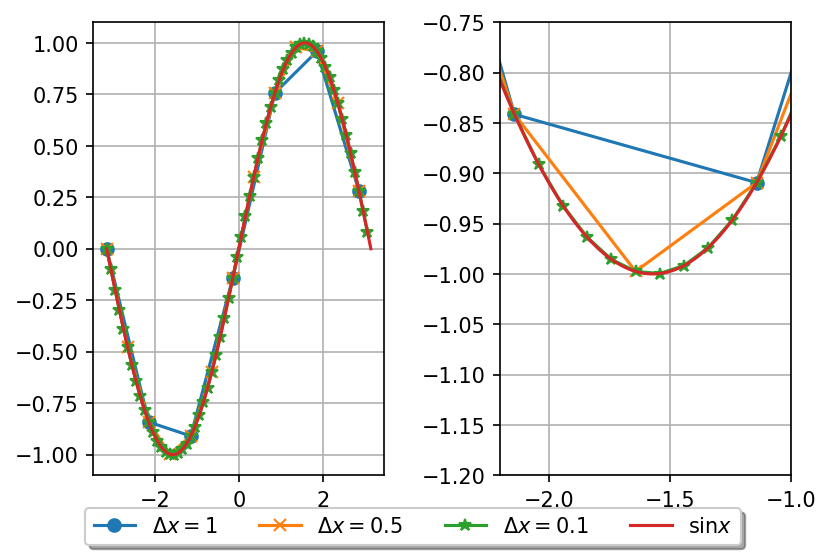
\includegraphics[width=0.9\linewidth]{fig-taylor/func_plot.png}}
  \caption{
  A plot of $\sin x$ for different spacing of the $x$-values. \label{fig:taylor:sinx}
  }
\end{figure}
%\clearpage % flush figures fig:taylor:sinx


From the figure we see that in some areas only a couple of points are needed in order to
represent the function well, and in some areas more points are needed. To state it more clearly; between $[-1,1]$ a linear function (few points) approximate $\sin x$ well, 
whereas in the area where the derivative of the function changes e.g.~in $[-2,-1]$, we need the points to be more closely spaced to capture the behavior of the true function.



\begin{graybox2admon}[Discretization]
To represent a function of space and/or time in a computer, the function needs to be discretized. When a function is discretized it leads to discretization errors.
\end{graybox2admon}




Why do we care about the number of points? In many cases the function we would like to evaluate can take a very long time to evaluate. Sometimes simulation time is not an issue, then we can use a large number of function
evaluations. However, in many applications simulation time \emph{is an issue}, and it would be good to know where the points needs to be closely spaced, and where we can 
manage with only a few points.

What is a \emph{good representation} representation of the true function? We cannot rely on visual inspection. In the next section we will show how Taylor polynomial representation of a function is a natural starting point to answer this question.

\section{Taylor Polynomial Approximation}
There are many ways of representing a function, but perhaps one of the most widely used is Taylor polynomials. 
Taylor series are the basis for solving ordinary and differential equations, simply because it makes it possible to evaluate any function with a set
of limited operations: \emph{addition, subtraction, and multiplication}. The Taylor polynomial, $P_n(x)$ of degree $n$ of a function $f(x)$ at the point $c$ is defined as:


\begin{graybox2admon}[Taylor polynomial:]

\begin{align}
 P_n(x) &= f(c)+f^\prime(c)(x-c)+\frac{f^{\prime\prime}(c)}{2!}(x-c)^2+\cdots+\frac{f^{(n)}(c)}{n!}(x-c)^n\nonumber\\ 
&=\sum_{k=0}^n\frac{f^{(n)}(c)}{k!}(x-c)^k.\label{eq:taylor:taylori}
\end{align}
\end{graybox2admon}



If the series is around the point $c=0$, the Taylor polynomial $P_n(x)$ is often called a Maclaurin polynomial, more examples can be found 
\href{{https://en.wikipedia.org/wiki/Taylor_series}}{here}\footnote{\texttt{https://en.wikipedia.org/wiki/Taylor\_series}}. If the series converge (i.e.~that the higher order terms approach zero), then we can represent the
function $f(x)$ with its corresponding Taylor series around the point $x=c$:
\begin{align}
 f(x) &= f(c)+f^\prime(c)(x-c)+\frac{f^{\prime\prime}(c)}{2!}(x-c)^2+\cdots
=\sum_{k=0}^\infty\frac{f^{(n)}}{k!}(x-c)^k.\label{eq:taylor:taylor}
\end{align}
The Maclaurin series of $\sin x$ is:
\begin{align}
\sin x = x-\frac{x^3}{3!}+\frac{x^5}{5!}-\frac{x^7}{7!}+\cdots=\sum_{k=0}^{\infty}\frac{(-1)^n}{(2n+1)!}x^{2n+1}.
\label{sin}
\end{align}

In figure~\ref{fig:mac_sin}, we show the first nine terms in the Maclaurin series for $\sin x$ (all even terms are zero). 

\begin{figure}[!ht]  % fig:mac_sin
  \centerline{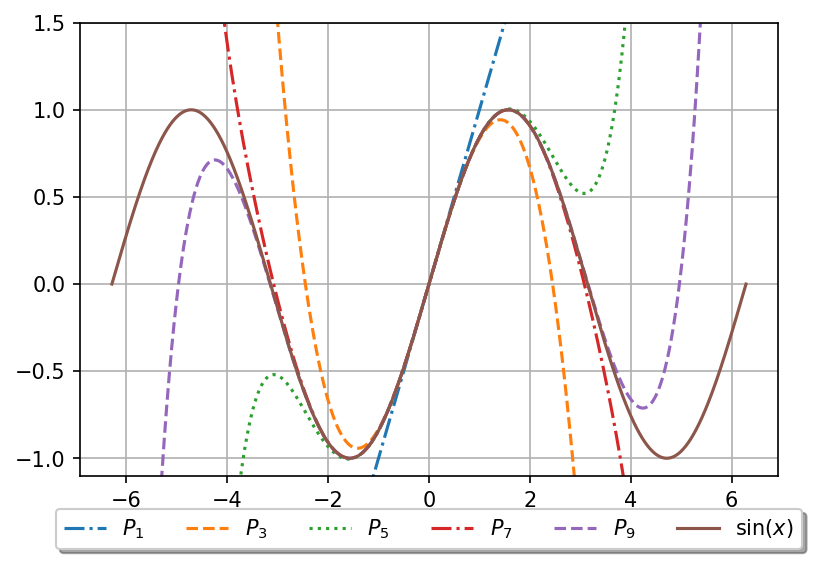
\includegraphics[width=0.9\linewidth]{fig-taylor/mac_sin.png}}
  \caption{
  Up to ninth order in the Maclaurin series of $\sin x$. \label{fig:mac_sin}
  }
\end{figure}
%\clearpage % flush figures fig:mac_sin

Note that we get a decent representation of $\sin x$ on the domain, by \emph{only knowing the function and its derivative in a single point}. 
The error term in Taylors formula, when we represent a function with a finite number of polynomial elements is given by:


\begin{graybox2admon}[Error term in Taylors formula:]
\begin{align}
R_n(x)&=f(x)-P_n(x)=\frac{f^{(n+1)}(\eta)}{(n+1)!}(x-c)^{n+1}\nonumber\\ 
      &=\frac{1}{n!}\int_c^x(x-\tau)^{n}f^{(n+1)}(\tau)d\tau,\label{eq:taylor:error}
\end{align}
for some $\eta$ in the domain $[x,c]$.
\end{graybox2admon}



If we want to calculate 
$\sin x$ to a precision lower than a specified value we can do it as follows:

\begin{lstlisting}[language=Python,style=blue1bar]
import numpy as np

# Sinus implementation using the Maclaurin Serie
# By setting a value for eps this value will be used
# if not provided
def my_sin(x,eps=1e-16):
    f = power = x
    x2 = x*x
    sign = 1
    i=0
    while(power>=eps):
        sign = - sign
        power *= x2/(2*i+2)/(2*i+3)
        f += sign*power
        i += 1
    print('No function evaluations: ', i)
    return f

x=0.8
eps = 1e-9
print(my_sin(x,eps), 'error = ', np.sin(x)-my_sin(x,eps))
\end{lstlisting}

This implementation needs some explanation:

\begin{itemize}
\item The error term is given in equation (\ref{eq:taylor:error}), and it is a even power in $x$. We do not which $\eta$ to use in equation (\ref{eq:taylor:error}), thus we use a trick and simply say that the error term is smaller than the highest order term. Thus, we stop the evaluation if the highest order term in the series is lower than the uncertainty. Thus, in practice we add the error term to the function evaluation, our estimate will always be better than the specified accuracy.

\item We evaluate the polynomials in the Taylor series by using the previous values too avoid too many multiplications within the loop, we do this by using the following identity:
\end{itemize}

\noindent
  \begin{align}
  \sin x&=\sum_{k=0}^{\infty} (-1)^nt_n, \text{ where: } t_n\equiv\frac{x^{2n+1}}{(2n+1)!}, \text{ hence :}\nonumber\\ 
  t_{n+1}&=\frac{x^{2(n+1)+1}}{(2(n+1)+1)!}=\frac{x^{2n+1}x^2}{(2n+1)! (2n+2)(2n+3)}\nonumber\\ 
  &=t_n\frac{x^2}{(2n+2)(2n+3)}
  \end{align}

\subsection{Evaluation of polynomials}
How to evaluate a polynomial of the type: $p_n(x)=a_0+a_1x+a_2x^2+\cdots+a_nx^n$? We already saw a hint in the previous section that it can be done in different ways. One way is simply to 
do:
\begin{lstlisting}[language=Python,style=blue1]
pol = a[0]
for i in range(1,n+1):
	pol = pol + a[i]*x**i
\end{lstlisting}
Note that there are $n$ additions, whereas there are $1 + 2 +3+\cdots+n=n(n+1)/2$ multiplications for all the iterations. Instead of evaluating the powers all over in 
each loop, we can use the previous calculation to save the number of multiplications:
\begin{lstlisting}[language=Python,style=blue1]
pol = a[0] + a[1]*x
power = x
for i in range(2,n+1):
	power  = power*x
	pol    = pol + a[i]*power
\end{lstlisting}
In this case there are still $n$ additions, but now there are $2n-1$ multiplications. For $n=15$, this amounts to 120 for the first, and 29 for the second method. 
Polynomials can also be evaluated using \emph{nested multiplication}:
\begin{align}
p_1 & = a_0+a_1x\nonumber\\ 
p_2 & = a_0+a_1x+a_2x^2=a_0+x(a_1+a_2x)\nonumber\\ 
p_3 & = a_0+a_1x+a_2x^2+a_3x^3=a_0+x(a_1+x(a_2+a_3x))\nonumber\\ 
\vdots
\end{align}   
and so on. This can be implemented as:
\begin{lstlisting}[language=Python,style=blue1]
pol = a[n]
for i in range(n-1,1,-1):
	pol  = a[i] + pol*x
\end{lstlisting}
In this case we only have $n$ multiplications. So if you know beforehand exactly how many terms is needed to calculate the series, this method would be the preferred method, and is implemented in NumPy as \href{{https://docs.scipy.org/doc/numpy/reference/generated/numpy.polyval.html#r138ee7027ddf-1}}{\nolinkurl{polyval}\footnote{\texttt{https://docs.scipy.org/doc/numpy/reference/generated/numpy.polyval.html\#r138ee7027ddf-1}}}. 

\section{Calculating Derivatives of Functions}
\label{ch:taylor:der}

index{forward difference}


The derivative of a function can be calculated using the definition from calculus:
\begin{align}
f^\prime(x)=\lim_{h\to 0}\frac{f(x+h)-f(x)}{h}\simeq \frac{f(x+h)-f(x)}{h}.\label{eq:taylor:der1}
\end{align}  
Not that $h$ can be both positive and negative, if $h$ is positive equation (\ref{eq:taylor:der1}) is termed \emph{forward difference}, because we use the function value on the right ($f(x+|h|)$). If on the other hand $h$ is negative equation (\ref{eq:taylor:der1}) is termed \emph{backward difference}, because we use the value to the left ($f(x-|h|)$). ($|h|$ is the absolute value of $h$).
In the computer we cannot take the limit, $h\to 0$, a natural question is then: What value to use for $h$? 
In figure~\ref{fig:taylor:df}, we have evaluated the numerical derivative of $\sin x$, using the formula in equation (\ref{eq:taylor:der1}) for different step sizes $h$. 

\begin{figure}[!ht]  % fig:taylor:df
  \centerline{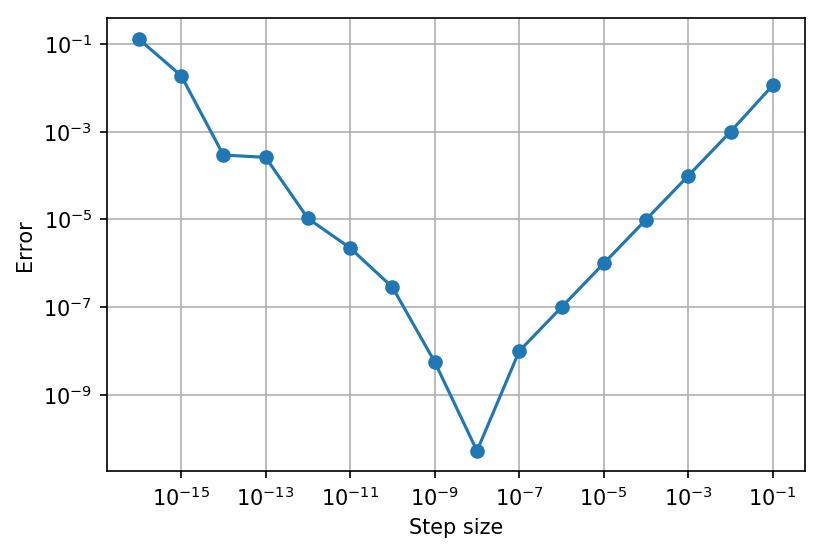
\includegraphics[width=0.9\linewidth]{fig-taylor/df.png}}
  \caption{
  Error in the numerical derivative of $\sin x$ at $x=0.2$ for different step size. \label{fig:taylor:df}
  }
\end{figure}
%\clearpage % flush figures fig:taylor:df



We clearly see that the error depends on the step size, but there is a minimum; choosing a step size too large give a poor estimate and choosing a too low step size give an 
even worse estimate. The explanation for this behavior is two competing effects: \emph{mathematical approximation} and \emph{round off errors}. Let us consider approximation or truncation error
first. By using the Taylor expansion in equation (\ref{eq:taylor:taylor}) and expand about $x$ and the error formula (\ref{eq:taylor:error}), we get:
\begin{align}
f(x+h)&=f(x)+f^\prime(x)h + \frac{h^2}{2}f^{\prime\prime}(\eta)\text{ , hence:}\nonumber\\ 
f^\prime(x)&=\frac{f(x+h)-f(x)}{h}-\frac{h}{2}f^{\prime\prime}(\eta),\label{eq:taylor:derr}
\end{align}
for some $\eta$ in $[x,x+h]$. Thus the error to our approximation is $hf^{\prime\prime}(\eta)/2$, if we reduce the step size by a factor of 10 the error is reduced by a factor of 10. 
Inspecting the graph, we clearly see that this is correct as the step size decreases from $10^{-1}$ to $10^{-8}$. When the step size decreases more, there is an increase in the error. This
is due to round off errors, and can be understood by looking into how numbers are stored in a computer.  

\subsection{Big $\mathcal{O}$ notation}
\href{{https://rob-bell.net/2009/06/a-beginners-guide-to-big-o-notation/}}{example}\footnote{\texttt{https://rob-bell.net/2009/06/a-beginners-guide-to-big-o-notation/}}

\subsection{Round off Errors}
In a computer a floating point number,$x$, is represented as:
\begin{align}
x=\pm q2^m.
\end{align}
Most computers are 64-bits, then one bit is reserved for the sign, 52 for the fraction ($q$) and 11 for
the exponent ($m$)  (for a graphic illustration see \href{{https://en.wikipedia.org/wiki/Double-precision_floating-point_format}}{Wikipedia}\footnote{\texttt{https://en.wikipedia.org/wiki/Double-precision\_floating-point\_format}}).
what is the largest \emph{floating point} number the computer can represent? 
Since $m$ contains 11 bits, $m$ can have the maximal value $m=2^{11}=1024$, and then the largest value is close to $2^{1024}\simeq 10^{308}$.
If you enter \texttt{print(10.1*10**(308))} in Python the answer will be \texttt{Inf}. If you enter \texttt{print(10*10**(308))}, Python will give an answer. This is because 
the number $10.1\cdot10^{308}$ is floating point number, whereas $10^{309}$ is an \emph{integer}, and Python does something clever when it comes to representing integers. 
Python has a third numeric type called long int, which can use the available memory to represent an integer. 

$10^{308}$ is the largest number, but what is the highest precision we can use, or how many decimal places can we use for a floating point number? 
Since there are 52 bits for the fraction, there are $1/2^{52}\simeq10^{-16}$ decimal places. As an example
the value of $\pi$ is $3.14159265358979323846264338\ldots$, but in Python it can only be represented by 16 digits: $3.141592653589793$. In principle 
it does not sound so bad to have an answer accurate to 16 digits, and it is much better than most experimental results. 
So what is the problem? One problem that you should be aware of is that round off errors can be a serious problem when we subtract two numbers that 
are very close to one another. If we implement the following program in Python:
\begin{lstlisting}[language=Python,style=blue1]
h=1e-16
x = 2.1 + h
y = 2.1 - h
print((x-y)/h)
\end{lstlisting}
we expect to get the answer 2, but instead we get zero. By changing $h$ to a higher value, the answer will get closer to 2. 

Armed with this knowledge of round off errors, we can continue to analyze
the result in figure~\ref{fig:taylor:df}.
The round off error when we represent a floating point number $x$ in the 
machine will be of the order $x/10^{16}$ (\emph{not} $10^{-16}$). In general, when we evaluate a function the error will be of the order 
$\epsilon|f(x)|$, where $\epsilon\sim10^{-16}$. Thus equation (\ref{eq:taylor:derr}) is modified in the following way when we take into account the round off errors:
\begin{align}
f^\prime(x)=\frac{f(x+h)-f(x)}{h}\pm\frac{2\epsilon|f(x)|}{h}-\frac{h}{2}f^{\prime\prime}(\eta),\label{eq:taylor:derr2}
\end{align}
we do not know the sign of the round off error, so the total error $R_2$ is:
\begin{align}
R_2=\frac{2\epsilon|f(x)|}{h}+\frac{h}{2}|f^{\prime\prime}(\eta)|.\label{eq:taylor:derr3}
\end{align}
We have put absolute values around the function and its derivative to get the maximal error, it might be the case that the round off error cancel part of the 
truncation error. However, the round off error is random in nature and will change from machine to machine, and each time we run the program. 
Note that the round off error increases when $h$ decreases, and the approximation error decreases when $h$ decreases. This is exactly what we see in the figure above. We can find the 
best step size, by differentiating $R_2$ and put it equal to zero:
\begin{align}
\frac{dR_2}{dh}&=-\frac{2\epsilon|f(x)|}{h^2}+\frac{1}{2}f^{\prime\prime}(\eta)=0\nonumber\\ 
h&=2\sqrt{\epsilon\left|\frac{f(x)}{f^{\prime\prime}(\eta)}\right|}\simeq 2\cdot10^{-8},\label{eq:taylor:derr4}
\end{align}
In the last equation we have assumed that $f(x)$ and its derivative is $~1$. This step size corresponds to an error of order $R_2\sim10^{-8}$. 
Inspecting 
the result in figure~\ref{fig:taylor:df}.
we see that the minimum is located at $h\sim10^{-8}$.      

\section{Higher Order Derivatives}
There are more ways to calculate the derivative of a function, than the formula given in equation (\ref{eq:taylor:derr}). Different formulas can be
derived by using Taylors formula in (\ref{eq:taylor:taylor}), usually one expands about $x\pm h$:
\begin{align}
f(x+h)&=f(x)+f^\prime(x)h + \frac{h^2}{2}f^{\prime\prime}(x)+ \frac{h^3}{3!}f^{(3)}(x)+ \frac{h^4}{4!}f^{(4)}(x)+\cdots\nonumber\\ 
f(x-h)&=f(x)-f^\prime(x)h + \frac{h^2}{2}f^{\prime\prime}(x)- \frac{h^3}{3!}f^{(3)}(x)+ \frac{h^4}{4!}f^{(3)}(x)-\cdots.
\end{align}
If we add these two equations, we get an expression for the second derivative, because the first derivative cancels out. But we also observe that if we subtract these two equations we get 
an expression for the first derivative that is accurate to a higher order than the formula in equation (\ref{eq:taylor:der1}), hence:
\begin{align}
f^\prime(x)&=\frac{f(x+h)-f(x-h)}{2h} -\frac{h^2}{6}f^{(3)}(\eta),\label{eq:taylor:der2}\\ 
f^{\prime\prime}(x) &= \frac{f(x+h)+f(x-h)-2f(x)}{h^2}+ \frac{h^2}{12}f^{(4)}(\eta)\label{eq:taylor:2der},
\end{align}
for some $\eta$ in $[x,x+h]$. In figure~\ref{fig:taylor:df2}, we have plotted equation (\ref{eq:taylor:derr}), (\ref{eq:taylor:der2}), and (\ref{eq:taylor:2der}) for 
different step sizes. The derivative in equation (\ref{eq:taylor:der2}), gives a higher accuracy than equation (\ref{eq:taylor:derr}) for a larger step size,
as can bee seen in figure~\ref{fig:taylor:df2}.


\begin{figure}[!ht]  % fig:taylor:df2
  \centerline{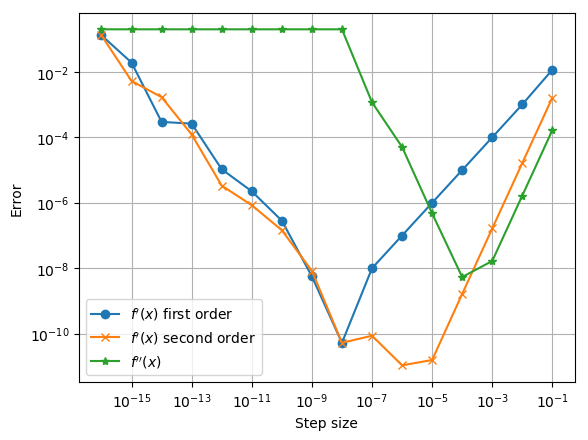
\includegraphics[width=0.9\linewidth]{fig-taylor/df2.png}}
  \caption{
  Error in the numerical derivative and second derivative of $\sin x$ at $x=0.2$ for different step size. \label{fig:taylor:df2}
  }
\end{figure}
%\clearpage % flush figures fig:taylor:df2


We can perform a similar error analysis as we did before, and then we find for equation (\ref{eq:taylor:der2}) and (\ref{eq:taylor:2der}) that the total
numerical error is:
\begin{align}
R_3&=\frac{\epsilon|f(x)|}{h}+\frac{h^2}{6}f^{(3)}(\eta),\label{eq:taylor:derr3b}\\ 
R_4&=\frac{4\epsilon|f(x)|}{h^2}+\frac{h^2}{12}f^{(4)}(\eta),\label{eq:taylor:derr4b}
\end{align}
respectively. Differentiating these two equations with respect to $h$, and set the equations equal to zero, we find an optimal step size of
$h\sim10^{-5}$ for equation (\ref{eq:taylor:derr3b}), which gives an error of $R_2\sim 10^{-16}/10^{-5}+(10^{-5})^2/6\simeq10^{-10}$, and $h\sim10^{-4}$ for equation
(\ref{eq:taylor:derr4b}), which gives an error of $R_4\sim 4\cdot10^{-16}/(10^{-4})^2+(10^{-4})^2/12\simeq10^{-8}$. Note that we get the surprising result for the first order 
derivative in equation (\ref{eq:taylor:der2}), that a higher step size gives a more accurate result. 







% !split
\chapter{Linear and nonlinear equations}
\label{ch:nlin}
Solving systems of equations are one of the most common tasks that we use computers for within modeling. A typical task is that we have have a model that contains a set of unknown parameters which we want to determine. To determine these parameters we need to solve a set of equations. In many cases these equations are nonlinear, but often a nonlinear problem is solved
\emph{by linearize} the nonlinear equations, and thereby reducing it to a sequence of linear algebra problems. Thus the topic of solving linear systems of equations have been extensively studied, and sophisticated linear equation solving packages have been developed. Python uses functions from the \href{{https://en.wikipedia.org/wiki/LAPACK}}{LAPACK}\footnote{\texttt{https://en.wikipedia.org/wiki/LAPACK}} library. In this course we will only cover the theory behind numerical linear algebra superficially, and the main purpose is to shed some light on some of the challenges one might encounter solving linear systems. In particular it is important for you to understand when it is stated in the NumPy documentation that the standard linear solver: \href{{https://docs.scipy.org/doc/numpy/reference/generated/numpy.linalg.solve.html}}{\nolinkurl{solve}\footnote{\texttt{https://docs.scipy.org/doc/numpy/reference/generated/numpy.linalg.solve.html}}} function uses \emph{LU-decomposition} and \emph{partial pivoting}. 

After covering some basics of numerical linear algebra, we will shift focus to nonlinear equations. Contrary to linear equations, you will most likely find that the functions available in various Python library will \emph{not} cover your needs and in many cases fail to give you the correct solution. The reason for this is that the solution of a nonlinear equation is greatly dependent on the starting point, and a combination of various techniques must be used.  

\section{Solving linear equations}
There are a number of excellent books covering this topic, see e.g.~\cite{press2007,trefethen1997,stoer2013,strang2019}.
In most of the examples covered in this course we will encounter problems where we have a set of \emph{linearly independent} equations and one equation for each unknown. For these type of problems there are a number of methods that can be used, and they will find a solution in a finite number of steps. If a solution cannot be found it is usually because the equations are not linearly independent, and our formulation of the physical problem is wrong.

Assume that we would like to solve the following set of equations:
\begin{align}
2x_0+x_1+x_2+3x_3&=1,\label{eq:nlin:la} \\ 
x_0+x_1+3x_2+x_3&=-3,\label{eq:nlin:lb} \\ 
x_0+4x_1+x_2+x_3&=2,\label{eq:nlin:lc} \\ 
x_0+x_1+x_2+x_3&=1.\label{eq:nlin:ld} 
\end{align}
These equations can be written in matrix form as:
\begin{equation}
\mathbf{A\cdot x}=\mathbf{b},
\label{eq:nlin:mat}
\end{equation}
where:
\begin{equation}
\mathbf{A}\equiv\begin{pmatrix}
2&1&1&3\\ 
1&1&3&1\\ 
1&4&1&1\\ 
1&1&2&2
\end{pmatrix}
\qquad
\mathbf{b}\equiv
\begin{pmatrix}
1\\-3\\2\\1
\end{pmatrix}
\qquad
\mathbf{x}\equiv
\begin{pmatrix}
x_0\\x_1\\x_2\\x_3
\end{pmatrix}.
\label{eq:nlin:matA}
\end{equation}
You can easily verify that $x_0=-4, x_1=1, x_2=-1, x_3= 3$ is the solution to the above equations by direct substitution. If we were to replace one of the above equations with a linear combination of any of the other equations, e.g.~replace equation (\ref{eq:nlin:ld}) with $3x_0+2x_1+4x_2+4x_3=-2$, there would be no solution. This can be checked by calculating the determinant of the matrix $\mathbf{A}$, if $\det \mathbf{A}=0 $,  
What is the difficulty in solving these equations? Clearly if none of the equations are linearly dependent, and we have $N$ independent linear equations, it should be straight forward to solve them? Two major numerical problems are i) even if the equations are not exact linear combinations of each other, they could be very close, and as the numerical algorithm progresses they could at some stage become linearly dependent due to roundoff errors. ii) roundoff errors may accumulate if the number of equations are large \cite{press2007}.

\subsection{Gauss-Jordan elimination}
Let us continue the discussion by consider Gauss-Jordan elimination, which is a \emph{direct} method. A direct method uses a final set of operations to obtain a solution. According to \cite{press2007} Gauss-Jordan elimination is the method of choice if we want to find the inverse of $\mathbf{A}$. However, it is slow when it comes to calculate the solution of equation
(\ref{eq:nlin:mat}). Even if speed and memory use is not an issue, it is also not advised to first find the inverse, $\mathbf{A}^{-1}$, of $\mathbf{A}$, then multiply it with $\mathbf{b}$ to obtain the solution, due to roundoff errors (Roundoff errors occur whenever we subtract to numbers that are very close to each other). To simplify our notation, we write equation (\ref{eq:nlin:matA}) as:
\begin{equation}
\left(
\begin{array}{cccc|c}
2&1&1&3&1\\ 
1&1&3&1&-3\\ 
1&4&1&1&2\\ 
1&1&2&2&1
\end{array}
\right).
\end{equation}
The numbers to the left of the vertical dash is the matrix $\mathbf{A}$, and to the right is the vector $\mathbf{b}$. The Gauss-Jordan elimination procedure proceeds by doing the same operation on the right and left side of the dash, and the goal is to get only zeros on the lower triangular part of the matrix. This is achieved by multiplying rows with the same (nonzero) number, swapping rows, adding a multiple of a row to another:
\begin{align}
&\left(
\begin{array}{cccc|c}
2&1&1&3&1\\ 
1&1&3&1&-3\\ 
1&4&1&1&2\\ 
1&1&2&2&1
\end{array}
\right)\to
\left(
\begin{array}{cccc|c}
2&1&1&3&1\\ 
0&1/2&5/2&-1/2&-7/2\\ 
0&7/2&1/2&-1/2&3/2\\ 
0&1/2&3/2&1/2&1/2
\end{array}
\right)\to\label{eq:nlin:gj1}\\ 
&\left(
\begin{array}{cccc|c}
2&1&1&3&1\\ 
0&1/2&5/2&-1/2&-7/2\\ 
0&0&-17&3&26\\ 
0&0&1&-1&4
\end{array}
\right)
\to
\left(
\begin{array}{cccc|c}
2&1&1&3&1\\ 
0&1/2&5/2&-1/2&-7/2\\ 
0&0&-17&3&26\\ 
0&0&0&14/17&42/17
\end{array}
\right)\no
\end{align}
The operations done are: ($1\to2$) multiply first row with $-1/2$ and add to second, third and the fourth row, ($2\to 3$) multiply second row with $-7$, and add to third row, multiply second row with $-1$ and add to fourth row, ($3\to4$) multiply third row with $-1/17$ and add to fourth row. These operations can easily be coded into Python:
\begin{lstlisting}[language=Python,style=blue1]
A = np.array([[2, 1, 1, 3,],[1, 1, 3, 1],
              [1, 4, 1, 1, ],[1, 1, 2, 2 ]],float)
b = np.array([1,-3,2,1],float)
N=4
# Gauss-Jordan Elimination
for i in range(1,N):
    fact    = A[i:,i-1]/A[i-1,i-1]
    A[i:,] -= np.outer(fact,A[i-1,])
    b[i:]  -= b[i-1]*fact
\end{lstlisting}
Notice that the final matrix has only zeros beyond the diagonal, such a matrix is called \emph{upper triangular}. We still have not found the final solution, but from an upper triangular (or lower triangular) matrix it is trivial to determine the solution. The last row immediately gives us $14/17z=42/17$ or $z=3$, now we have the solution for z and the next row gives: $-17y+3z=26$ or $y=(26-3\cdot3)/(-17)=-1$, and so on. In a more general form, we can write our solution of the matrix $\mathbf{A}$ after making it upper triangular as:
\begin{equation}
\begin{pmatrix}
a^\prime_{0,0}&a^\prime_{0,1}&a^\prime_{0,2}&a^\prime_{0,3}\\ 
0&a^\prime_{1,1}&a^\prime_{1,2}&a^\prime_{1,3}\\ 
0&0&a^\prime_{2,2}&a^\prime_{2,3}\\ 
0&0&0&a^\prime_{3,3}
\end{pmatrix}
\cdot
\begin{pmatrix}
x_0\\ 
x_1\\ 
x_2\\ 
x_3
\end{pmatrix}
=
\begin{pmatrix}
b^\prime_{0}\\ 
b^\prime_{1}\\ 
b^\prime_{2}\\ 
b^\prime_{3}
\end{pmatrix}
\label{eq:nlin:back}
\end{equation}
The backsubstitution can then be written formally as:
\begin{equation}
x_i=\frac{1}{a^\prime_{ii}}\left[b_i^\prime-\sum_{j=i+1}^{N-1}a^\prime_{ij}x_j\right],\quad i=N-1,N-2,\ldots,0
\label{eq:nlin:back2}
\end{equation}
The backsubstitution can now easily be implemented in Python as:
\begin{lstlisting}[language=Python,style=blue1]
# Backsubstitution
sol = np.zeros(N,float)
sol[N-1]=b[N-1]/A[N-1,N-1]
for i in range(2,N+1):
    sol[N-i]=(b[N-i]-np.dot(A[(N-i),],sol))/A[N-i,N-i]
\end{lstlisting}
Notice that in the Python implementation, we have used vector operations instead of for loops. This makes the code more efficient, but it could also be implemented with for loops: 
\begin{lstlisting}[language=Python,style=blue1]
# Backsubstitution - for loop
sol = np.zeros(N,float)
for i in range(N-1,-1,-1):
    sol[i]= b[i]
    for j in range(i+1,N):
        sol[i] -= A[i][j]*sol[j]
    sol[i] /= A[i][i]
\end{lstlisting}
There are at least two things to notice with our implementation:
\begin{itemize}
\item Matrix and vector notation makes the code more compact and efficient. In order to understand the implementation it is advised to put $i=1, 2, 3, 4$, and then execute the statements in the Gauss-Jordan elimination and compare with equation (\ref{eq:nlin:gj1}).

\item The implementation of the Gauss-Jordan elimination is not robust, in particular one could easily imagine cases where one of the leading coefficients turned out as zero, and the routine would fail when we divide by \texttt{A[i-1,i-1]}. By simply changing equation (\ref{eq:nlin:lb}) to $2x_0+x_1+3x_2+x_3=-3$, when doing the first Gauss-Jordan elimination, both $x_0$ and $x_1$ would be canceled. In the next iteration we try to divide next equation by the leading coefficient of $x_1$, which is zero, and the whole procedure fails.
\end{itemize}

\noindent
\subsection{Pivoting}
The solution to the last problem is solved by what is called \emph{pivoting}. The element that we divide on is called the \emph{pivot element}. It actually turns out that even if we do Gauss-Jordan elimination \emph{without} encountering a zero pivot element, the Gauss-Jordan procedure is numerically unstable in the presence of roundoff errors \cite{press2007}. There are two versions of pivoting, \emph{full pivoting} and \emph{partial pivoting}. In partial pivoting we only interchange rows, while in full pivoting we also interchange rows and columns. Partial pivoting is much easier to implement, and the algorithm is as follows:
\begin{enumerate}
\item Find the row in $\mathbf{A}$ with largest absolute value in front of $x_0$ and change with the first equation, switch corresponding elements in $\mathbf{b}$

\item Do one Gauss-Jordan elimination, find the row in $\mathbf{A}$ with the largest absolute value in front of $x_1$ and switch with the second (same for $\mathbf{b}$), and so on.
\end{enumerate}

\noindent
For a linear equation we can multiply with a number on each side and the equation would be unchanged, so if we where to multiply one of the equations with a large value, we are almost sure that this equation would be placed first by our algorithm. This seems a bit strange as our mathematical problem is the same. Sometimes the linear algebra routines tries to normalize the equations to find the pivot element that would have been the largest element if all equations were normalized according to some rule, this is called \emph{implicit pivoting}.  
\subsection{LU decomposition}
As we have already seen, if the matrix $\mathbf{A}$ is reduced to a triangular form it is trivial to calculate the solution by using backsubstitution. Thus if it was possible to decompose the matrix $\mathbf{A}$ as follows:
\begin{align}
&\mathbf{A}=\mathbf{L}\cdot\mathbf{U}\label{eq:nlin:lu}\\ 
&\begin{pmatrix}
a_{0,0}&a_{0,1}&a_{0,2}&a_{0,3}\\ 
a_{1,0}&a_{1,1}&a_{1,2}&a_{1,3}\\ 
a_{2,0}&a_{2,0}&a_{2,2}&a_{2,3}\\ 
a_{3,0}&a_{3,0}&a_{3,0}&a_{3,3}
\end{pmatrix}
=
\begin{pmatrix}
l_{0,0}&0&0&0\\ 
l_{1,0}&l_{1,1}&0&0\\ 
l_{2,0}&l_{2,0}&l_{2,2}&0\\ 
l_{3,0}&l_{3,0}&l_{3,0}&l_{3,3}
\end{pmatrix}
\cdot
\begin{pmatrix}
u_{0,0}&u_{0,1}&u_{0,2}&u_{0,3}\\ 
0&u_{1,1}&u_{1,2}&u_{1,3}\\ 
0&0&u_{2,2}&u_{2,3}\\ 
0&0&0&u_{3,3}
\end{pmatrix}.\no
\end{align}
The solution procedure would then be to rewrite equation (\ref{eq:nlin:mat}) as:
\begin{align}
\mathbf{A\cdot x}=\mathbf{L}\cdot\mathbf{U}\cdot\mathbf{x}=\mathbf{b},\label{eq:nlin:matb}
\end{align}
If we define a new vector $\mathbf{y}$:
\begin{align}
\mathbf{y}\equiv\mathbf{U}\cdot\mathbf{x},
\end{align}
we can first solve for the $\mathbf{y}$ vector:
\begin{align}
\mathbf{L}\cdot\mathbf{y}=\mathbf{b},\label{eq:nlin:for}
\end{align}
and then for $\mathbf{x}$:
\begin{align}
\mathbf{U}\cdot\mathbf{x}=\mathbf{y}.
\end{align}
Note that the solution to equation (\ref{eq:nlin:for}) would be done by \emph{forward substitution}:
\begin{equation}
y_i=\frac{1}{l_{ii}}\left[b_i-\sum_{j=0}^{i-1}l_{ij}x_j\right],\quad i=1,2,\ldots N-1.
\label{eq:nlin:back3}
\end{equation}
Why go to all this trouble? First of all it requires (slightly) less operations to calculate the LU decomposition and doing the forward and backward substitution than the Gauss-Jordan procedure discussed earlier. Secondly, and more importantly, is the fact that in many cases one would like to calculate the solution for different values of the $\mathbf{b}$ vector in equation (\ref{eq:nlin:matb}). If we do the LU decomposition first we can calculate the solution quite fast using backward and forward substitution for any value of the $\mathbf{b}$ vector.

The NumPy function \href{{https://docs.scipy.org/doc/numpy/reference/generated/numpy.linalg.solve.html}}{\nolinkurl{solve}\footnote{\texttt{https://docs.scipy.org/doc/numpy/reference/generated/numpy.linalg.solve.html}}}, uses LU decomposition and partial pivoting, and we can find the solution to our previous problem simply by the following code:
\begin{lstlisting}[language=Python,style=blue1]
from numpy.linalg import solve
x=solve(A,b)
\end{lstlisting}

\section{Example: Linear regression}
In the previous section, we considered a system of $N$ equations and $N$ unknown ($x_0, x_1,\ldots, x_N$). In general we might have more equations than unknowns or more unknowns than equations. An example of the former is linear regression, we might have many data points and we would like to fit a line through the points. How do you fit a single lines to more than two points that does not line on the same line? One way to do it is to minimize the distance from the line to the points, as illustrated in figure~\ref{fig:nlin:reg}.

\begin{figure}[!ht]  % fig:nlin:reg
  \centerline{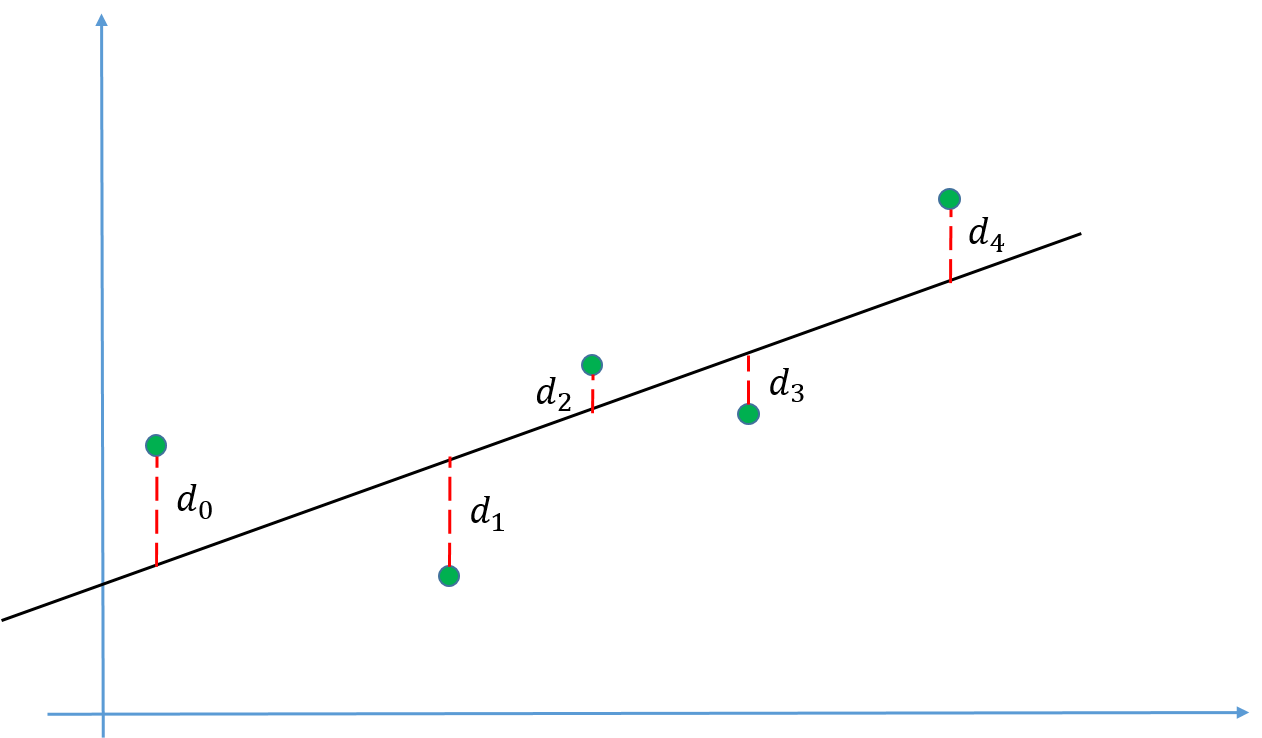
\includegraphics[width=0.5\linewidth]{fig-nlin/reg.png}}
  \caption{
  Linear regression by minimizing the total distance to all the points. \label{fig:nlin:reg}
  }
\end{figure}
%\clearpage % flush figures fig:nlin:reg

Mathematically we can express the distance between a data point $(x_i,y_i)$ and the line $f(x)$ as $y_i-f(x_i)$. Note that this difference can be negative or positive depending if the data point lies below or above the line. We can then take the absolute value of all the distances, and try to minimize them. When we minimize something we take the derivative of the expression and put it equal to zero.  As you might remember from Calculus it is extremely hard to work with the derivative of the absolute value, because it is discontinuous. A much better approach is to square each distance and sum them:
\begin{equation}
S=\sum_{i=0}^3(y_i-f(x_i))^2=\sum_{i=0}^3(y_i-a_0-a_1x_i)^2.
\label{eq:nlin:lsq}
\end{equation}
This is the idea behind \emph{least square}, and linear regression. One thing you should be aware of is that points lying far from the line will contribute more to equation (\ref{eq:nlin:lsq}). The underlying assumption is that each data point provides equally precise information about the process, this is often not the case. When analyzing experimental data, there may be points deviating from the expected behaviour, it is then important to investigate if these points are more affected by measurements errors than the others. If that is the case one should give them less weight in the least square estimate, by extending the formula above:
\begin{equation}
S=\sum_{i=0}^3\omega_i(y_i-f(x_i))^2=\sum_{i=0}^3\omega_i(y_i-a_0-a_1x_i)^2,
\label{eq:nlin:lsqm}
\end{equation}
$\omega_i$ is a weight factor.

Let us continue with equation (\ref{eq:nlin:lsq})

Two great explanations \href{{https://medium.com/@andrew.chamberlain/the-linear-algebra-view-of-least-squares-regression-f67044b7f39b}}{linear regression by
matrices}\footnote{\texttt{https://medium.com/@andrew.chamberlain/the-linear-algebra-view-of-least-squares-regression-f67044b7f39b}},
and 
\href{{https://medium.com/@andrew.chamberlain/a-more-elegant-view-of-r-squared-a0a14c177dc3}}{$R^2$-squared}\footnote{\texttt{https://medium.com/@andrew.chamberlain/a-more-elegant-view-of-r-squared-a0a14c177dc3}}

\section{Example: Solving the heat equation regression}

\section{Singular Value Decomposition}

\section{QR factorization}

\section{Solving nonlinear equations}
The purpose of this section is to introduce a handful of techniques for solving a nonlinear equation. In many cases a combination of methods must be used, and the algorithm must be adopted to your specific problem. 
% !split
\chapter{Numerical integration}
\label{ch:numint}



\section{Numerical Integration}
Before diving into the details of this section, it is worth pointing out that the derivation of the algorithms in this section follows a general pattern:

\begin{enumerate}
\item We start with a mathematical model (in this case an integral)

\item The mathematical model is formulated in discrete form 

\item Then we design an algorithm to solve the model 

\item The numerical solution for a test case is compared with the true solution (could be an analytical solution or data)

\item Error analysis: we investigate the accuracy of the algorithm by changing the number of iterations and/or make changes to the implementation or algorithm
\end{enumerate}

\noindent
In practice you would not use your own implementation to calculate an integral, but in order to understand which method to use 
in a specific case, it is important to understand the limitation and advantages of the different algorithms. The only way to achieve this is to 
have a basic understanding of the development. There might also be some cases where you would like to adapt an integration scheme to your specific
case if there is a special need  that the integration is fast. 

\subsection{The Midpoint Rule}
Numerical integration is encountered in numerous applications in physics and engineering sciences. 
Let us first consider the most simple case, a function $f(x)$, which is a function of one variable, $x$. The most straight forward way of calculating the area $\int_a^bf(x)dx$ is 
simply to divide the area under the function into $N$ equal rectangular slices with size $h=(b-a)/N$, as illustrated in figure~\ref{fig:numint:mid}. The area of one box is:
\begin{equation}
M(x_k,x_k+h)=f(x_k+\frac{h}{2}) h,\label{eq:numint:mid0}
\end{equation}
and the area of all the boxes is:
\begin{align}
I(a,b)&=\int_a^bf(x)dx\simeq\sum_{k=0}^{N-1}M(x_k,x_k+h)\nonumber\\ 
&=h\sum_{k=0}^{N-1}f(x_k+\frac{h}{2})=h\sum_{k=0}^{N-1}f(a+(k+\frac{1}{2})h).
\label{eq:numint:mid1}
\end{align}
Note that the sum goes from $k=0,1,\ldots,N-1$, a total of $N$ elements. We could have chosen to let the sum go from $k=1,2,\ldots,N$. 
In Python, C, C++ and many other programming languages the arrays start by indexing the elements from $0,1,\ldots$ to $N-1$, 
therefore we choose the convention of having the first element to start at $k=0$.


\begin{figure}[!ht]  % fig:numint:mid
  \centerline{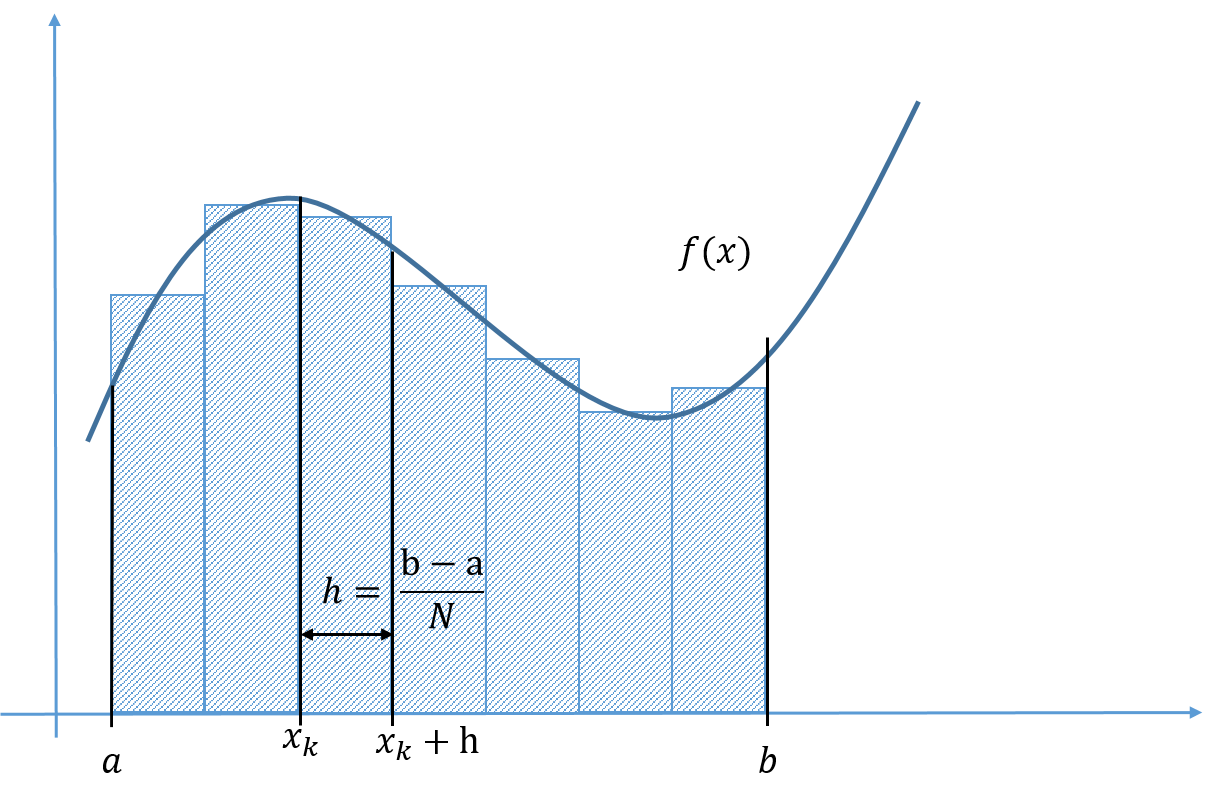
\includegraphics[width=0.9\linewidth]{fig-numint/func_sq.png}}
  \caption{
  Integrating a function with the midpoint rule. \label{fig:numint:mid}
  }
\end{figure}
%\clearpage % flush figures fig:numint:mid


Below is a Python code, where this algorithm is implemented for $\int_0^\pi\sin (x)dx$
\begin{lstlisting}[language=Python,style=blue1bar]
import numpy as np
# Function to be integrated
def f(x):
    return np.sin(x)

def int_midpoint(func, lower_limit, upper_limit,N):
    """ calculates the area of func over the domain lower_limit
        to upper limit using N integration points """
    h    = (upper_limit-lower_limit)/N # step size 
    area = 0.
    for all integration points do:
        estimate integration midpoint value, xi
        add area under curve: func(xi)*h
    return area
\end{lstlisting}


\begin{graybox2admon}[Notice]
There are many ways to calculate loops in a programming language. If you were coding in a lower level programming language like Fortran, C or C++, you would probably implement the loop like (in Python syntax):
\begin{lstlisting}[language=Python,style=blue1]
for k in range(0,N): # loop over k=0,1,..,N-1
    val = lower_limit+(k+0.5)*h # midpoint value
    area += func(val)
return area*h
\end{lstlisting}
However, in Python, you would always try to avoid loops because they are generally slow. A more efficient way of implementing the above rule would be to replace the loop with:
\begin{lstlisting}[language=Python,style=blue1]
val  = [lower_limit+(k+0.5)*h for k in range(N)]
ff   = func(val)
area = np.sum(ff)
return area*h
\end{lstlisting}
\end{graybox2admon}





\subsection{The Trapezoidal Rule}
The numerical error in the above example is quite low, only about 2$\%$ for $N=5$. 
However, by just looking at the graph above it seems likely that we can develop a better algorithm by using trapezoids instead of rectangles, 
see figure~\ref{fig:numint:trap}.


\begin{figure}[!ht]  % fig:numint:trap
  \centerline{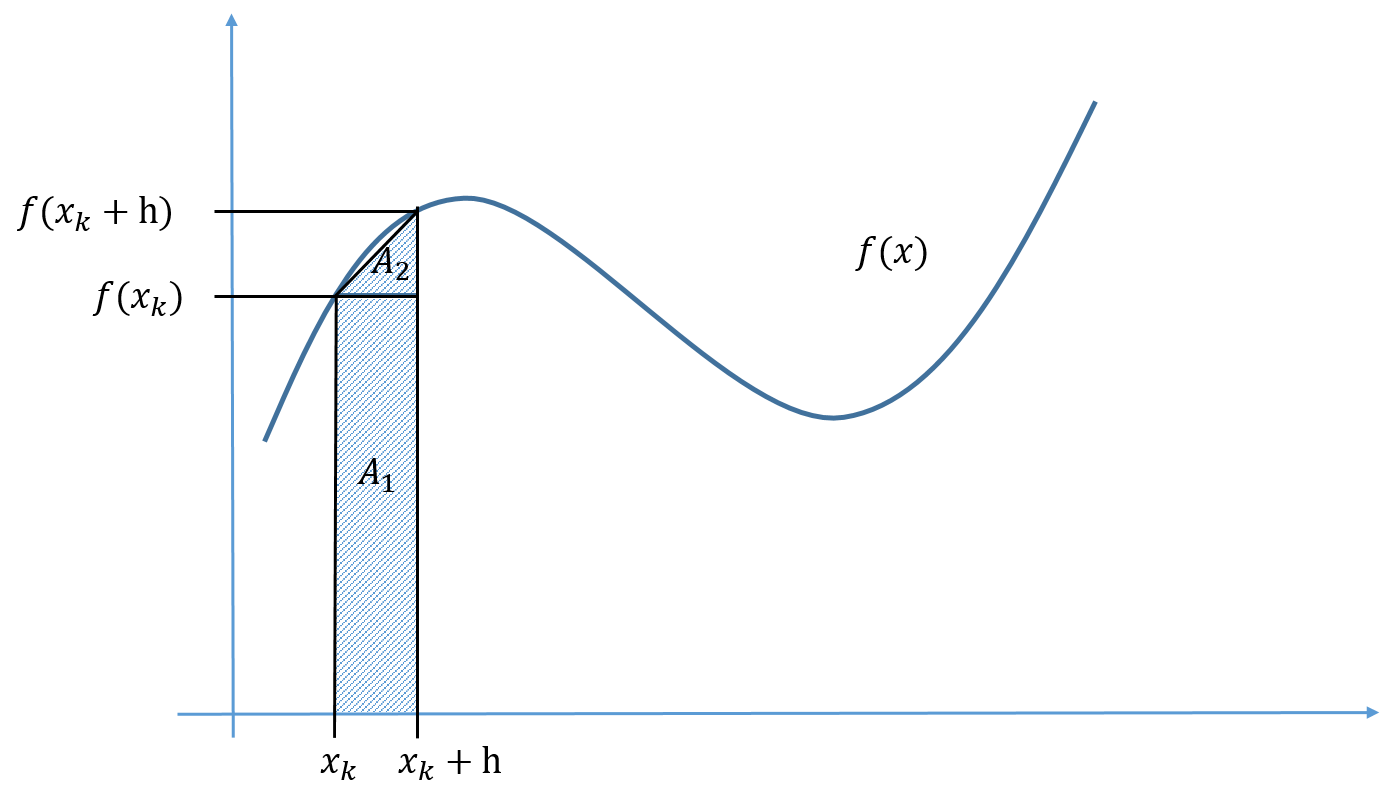
\includegraphics[width=0.9\linewidth]{fig-numint/func_tr.png}}
  \caption{
  Integrating a function with the trapezoidal rule. \label{fig:numint:trap}
  }
\end{figure}
%\clearpage % flush figures fig:numint:trap


Earlier we approximated the area using the midpoint value: $f(x_k+h/2)\cdot h$. Now we use $A=A_1+A_2$, where $A_1=f(x_k)\cdot h$ 
and $A_2=(f(x_k+h)-f(x_k))\cdot h/2$, hence the area of one trapezoid is:
\begin{equation}
A\equiv T(x_k,x_k+h)=(f(x_k+h)+f(x_k))h/2.
\end{equation}
This is the trapezoidal rule, and for the whole interval we get:
\begin{align}
I(a,b)&=\int_a^bf(x)dx\simeq\frac{1}{2}h\sum_{k=0}^{N-1}\left[f(x_k+k h)+f(x_k)\right] \nonumber \\ 
&=h\left[\frac{1}{2}f(a)+f(a+h) + f(a+2h) +\nonumber\right. \\ 
&\left.\qquad\cdots + f(a+(N-2)h)+\frac{1}{2}f(b)\right]\nonumber \\ 
&=h\left[\frac{1}{2}f(a)+\frac{1}{2}f(b)+\sum_{k=1}^{N-1}f(a+k h)\right].
\end{align}
Note that this formula was bit more involved to derive, but it requires only one more function evaluations compared to the midpoint rule. 
Below is a python implementation:
\begin{lstlisting}[language=Python,style=blue1bar]
import numpy as np
# Function to be integrated
def f(x):
    return np.sin(x)

#In the implementation below the calculation goes faster 
#when we avoid unnecessary multiplications by h in the loop
def int_trapez(func, lower_limit, upper_limit,N):
    """ calculates the area of func over the domain lower_limit
        to upper limit using N integration points """
    h       = (upper_limit-lower_limit)/N # step size
    area    = 0.5*(func(lower_limit)+func(upper_limit))
    val     = lower_limit
    for all integration points do:
        estimate integration midpoint value, xi
        add are under curve: func(xi)*h
    return area
\end{lstlisting}

In the table below, we have calculated the numerical error for various values of $N$.



{\small   % for Springer style: small table font and more vspace

\vspace{4mm}

\begin{tabular}{cccc}
\hline
\multicolumn{1}{c}{ $N$ } & \multicolumn{1}{c}{ $h$ } & \multicolumn{1}{c}{ Error Midpoint } & \multicolumn{1}{c}{ Error Trapezoidal } \\
\hline
1   & 3.14  & -57\%          & 100\%             \\
5   & 0.628 & -1.66\%        & 3.31\%            \\
10  & 0.314 & -0.412\%       & 0.824\%           \\
100 & 0.031 & -4.11E-3\%     & 8.22E-3\%         \\
\hline
\end{tabular}

\vspace{4mm}

}


\noindent

Note that we get the surprising result that this algorithm performs poorer, a factor of 2 than the midpoint rule.
How can this be explained? By just looking at figure~\ref{fig:numint:mid}, we see that the midpoint rule actually over predicts the area from $[x_k,x_k+h/2]$ 
 and under predicts in the interval $[x_k+h/2,x_{k+1}]$ or vice versa. The net effect is that for many cases the midpoint rule give a slightly better 
 performance than the trapezoidal rule. In the next section we will investigate this more formally.

\subsection{Numerical Errors on Integrals}
It is important to know the accuracy of the methods we are using, otherwise we do not know if the
computer produce correct results. In the previous examples we were able to estimate the error because we knew the analytical result. However, if we know the 
analytical result there is no reason to use the computer to calculate the result(!). Thus, we need a general method to estimate the error, and let the computer 
run until a desired accuracy is reached. 

In order to analyze the midpoint rule in more detail we approximate the function by a Taylor 
series at the midpoint between $x_k$ and $x_k+h$: 
\begin{align}
f(x)&=f(x_k+h/2)+f^\prime(x_k+h/2)(x-(x_k+h/2))\nonumber\\ 
&+\frac{1}{2!}f^{\prime\prime}(x_k+h/2)(x-(x_k+h/2))^2+\mathcal{O}(h^3)
\end{align}
Since $f(x_k+h/2)$ and its derivatives are constants it is straight forward to integrate $f(x)$:
\begin{align}
I(x_k,x_k+h)&=\int_{x_k}^{x_k+h}\left[f(x_k+h/2)+f^\prime(x_k+h/2)(x-(x_k+h/2))\right.\nonumber\\ 
&\left.+\frac{1}{2!}f^{\prime\prime}(x_k+h/2)(x-(x_k+h/2))^2+\mathcal{O}(h^3)\right]dx
\end{align}
The first term is simply the midpoint rule, to evaluate the two other terms we make the substitution: $u=x-x_k$:
\begin{align}
I(x_k,x_k+h)&=f(x_k+h/2)\cdot h+f^\prime(x_k+h/2)\int_0^h(u-h/2)du\nonumber\\ 
&+\frac{1}{2}f^{\prime\prime}(x_k+h/2)\int_0^h(u-h/2)^2du+\mathcal{O}(h^4)\nonumber\\ 
&=f(x_k+h/2)\cdot h-\frac{h^3}{24}f^{\prime\prime}(x_k+h/2)+\mathcal{O}(h^4).
\end{align}
Note that all the odd terms cancels out, i.e $\int_0^h(u-h/2)^m=0$ for $m=1,3,5\ldots$. Thus the error for the midpoint rule, $E_{M,k}$, on this particular interval is:
\begin{equation}
E_{M,k}=I(x_k,x_k+h)-f(x_k+h/2)\cdot h=-\frac{h^3}{24}f^{\prime\prime}(x_k+h/2),
\end{equation}
where we have ignored higher order terms. We can easily sum up the error on all the intervals, but clearly $f^{\prime\prime}(x_k+h/2)$ will 
not, in general, have the same value on all intervals. However, an upper bound for the error can be found by replacing $f^{\prime\prime}(x_k+h/2)$ 
with the maximal value on the interval $[a,b]$, $f^{\prime\prime}(\eta)$:
\begin{align}
E_{M}&=\sum_{k=0}^{N-1}E_{M,k}=-\frac{h^3}{24}\sum_{k=0}^{N-1}f^{\prime\prime}(x_k+h/2)\leq-\frac{Nh^3}{24}f^{\prime\prime}(\eta),\label{eq:numint:em}\\ 
E_{M}&\leq-\frac{(b-a)^3}{24N^2}f^{\prime\prime}(\eta),
\end{align}
where we have used $h=(b-a)/N$. We can do the exact same analysis for the trapezoidal rule, but then we expand the function around $x_k-h$ instead of the midpoint. 
The error term is then:
\begin{equation}
E_T=\frac{(b-a)^3}{12N^2}f^{\prime\prime}(\overline{\eta}).
\end{equation}
At the first glance it might look like the midpoint rule always is better than the trapezoidal rule, but note that the second derivative is 
evaluated in different points ($\eta$ and $\overline{\eta}$). Thus it is possible to construct examples where the midpoint rule performs poorer 
than the trapezoidal rule.

Before we end this section we will rewrite the error terms in a more useful form as it is not so easy to evaluate 
$f^{\prime\prime}(\eta)$ (since we do not know which value of $\eta$ to use). By taking a closer look at equation (\ref{eq:numint:em}), 
we see that it is closely related to the midpoint rule for $\int_a^bf^{\prime\prime}(x)dx$, hence:
\begin{align}
E_{M}&=-\frac{h^2}{24}h
\sum_{k=0}^{N-1}f^{\prime\prime}(x_k+h/2)\simeq-\frac{h^2}{24}\int_a^b
f^{\prime\prime}(x)dx\\ 
E_M&\simeq\frac{h^2}{24}\left[f^\prime(b)-f^\prime(a)\right]=-\frac{(b-a)^2}{24N^2}\left[f^\prime(b)-f^\prime(a)\right]
\end{align}
The corresponding formula for the trapezoid formula is:
\begin{equation}
E_T\simeq \frac{h^2}{12}\left[f^\prime(b)-f^\prime(a)\right]=\frac{(b-a)^2}{12N^2}\left[f^\prime(b)-f^\prime(a)\right]
\end{equation}
Now, we can make an algorithm that automatically choose the number of steps to reach (at least) a predefined accuracy:
\begin{lstlisting}[language=Python,style=blue1bar]
import numpy as np
# Function to be integrated
def f(x):
    return np.sin(x)
#Numerical derivative of function
def df(x,func):
    dh=1e-5 # some low step size
    return (func(x+dh)-func(x))/dh 
#Adaptive midpoint rule, "adaptive" because the number of 
#function evaluations depends on the integrand
def int_adaptive_midpoint(func, lower_limit, upper_limit, tol):
    """ calculates the area of func over the domain lower_limit
        to upper limit for the specified tolerance tol """
    dfa  = df(lower_limit,func) # derivative in point a 
    dfb  = df(upper_limit,func) # derivative in point b
    h    = np.sqrt(abs(24*tol/(dfb-dfa)))
    print('Number of intervals = ', (upper_limit-lower_limit)/h)
    for all integration points do:
        estimate integration midpoint value, xi
        add area under curve: func(xi)*h
    return area
\end{lstlisting}


\begin{graybox2admon}[Notice]
In Python it is sometimes convenient to enter default values for the arguments in a function. In the above example, we could also have written the function definition as\\ \Verb!def int_adaptive_midpoint(func, lower_limit, upper_limit,! \\ \texttt{tol=1e-8):}. If the \texttt{tol} parameter is not given the code will assume an accuracy of $10^{-8}$.
\end{graybox2admon}



\subsection{Practical Estimation of Errors on Integrals}
\label{sec:numint:parct}
From the example above we were able to estimate the number of steps needed to reach (at least) a certain precision. 
In many practical cases we do not deal with functions, but with data and it can be difficult to evaluate the derivative. 
We also saw from the example above that the algorithm gives a higher precision than what we asked for. 
How can we avoid doing too many iterations? A very simple solution to this question is to double the number of intervals until 
a desired accuracy is reached. The following analysis holds for both the trapezoid and midpoint method, because in both cases 
the error scale as $h^2$. 

Assume that we have evaluated the integral with a step size $h_1$, and the computed result is $I_1$. 
Then we know that the true integral is $I=I_1+c h_1^2$, where $c$ is a constant that is unknown. If we now half the step size: $h_2=h_1/2$, 
then we get a new (better) estimate of the integral, $I_2$, which is related to the true integral $I$ as: $I=I_2+c h_2^2$. 
Taking the difference between $I_2$ and $I_1$ give us an estimation of the error:
\begin{equation}
I_2-I_1=I-c h_2^2-(I-ch_1^2)=3c h_2^2,
\end{equation}
where we have used the fact that $h_1=2h_2$, Thus the error term is:
\begin{equation}
E(a,b)=c h_2^2=\frac{1}{3}(I_2-I_1).
\end{equation}
This might seem like we need to evaluate the integral twice as many times as needed. This is not the case, by choosing to exactly 
half the spacing we only need to evaluate for the values that lies halfway between the original points. We will demonstrate how 
to do this by using the trapezoidal rule, because it operates directly on the $x_k$ values and not the midpoint values. 
The trapezoidal rule can now be written as:
\begin{align}
I_2(a,b)&=h_2\left[\frac{1}{2}f(a)+\frac{1}{2}f(b)+\sum_{k=1}^{N_2-1}f(a+k h_2)\right],\\ 
&=h_2\left[\frac{1}{2}f(a)+\frac{1}{2}f(b)+\sum_{k=\text{even values}}^{N_2-1}f(a+k h_2)\right.\nonumber\\ 
&\left.\qquad+\sum_{k=\text{odd values}}^{N_2-1}f(a+k h_2)\right],
\end{align}
in the last equation we have split the sum into odd an even values. The sum over the even values can be rewritten:
\begin{equation}
\sum_{k=\text{even values}}^{N_2-1}f(a+k h_2)=\sum_{k=0}^{N_1-1}f(a+2k h_2)=\sum_{k=0}^{N_1-1}f(a+k h_1),
\end{equation}
note that $N_2$ is replaced with $N_1=N_2/2$, we can now rewrite $I_2$ as:
\begin{align}
I_2(a,b)&=h_2\left[\frac{1}{2}f(a)+\frac{1}{2}f(b)+\sum_{k=0}^{N_1-1}f(a+k h_1)\right.\nonumber\\ 
&\left.+\sum_{k=\text{odd values}}^{N_2-1}f(a+k h_2)\right]
\end{align}
Note that the first terms are actually the trapezoidal rule for $I_1$, hence:
\begin{equation}
I_2(a,b)=\frac{1}{2}I_1(a,b)+h_2\sum_{k=\text{odd values}}^{N_2-1}f(a+k h_2)
\end{equation}
A possible algorithm is then:
\begin{enumerate}
\item Choose a low number of steps to evaluate the integral, $I_0$, the first time, e.g.~$N_0=10$

\item Double the number of steps, $N_1=2N_0$ 

\item Calculate the missing values by summing over the odd number of steps $\sum_{k=\text{odd values}}^{N_1-1}f(a+k h_1)$

\item Check if $E_1(a,b)=\frac{1}{3}(I_1-I_0)$ is lower than a specific tolerance

\item If yes quit, if not, return to 2, and continue until $E_i(a,b)=\frac{1}{3}(I_{i+1}-I_{i})$ is lower than the tolerance  
\end{enumerate}

\noindent
Below is a Python implementation:
\begin{lstlisting}[language=Python,style=blue1bar]
import numpy as np
# Function to be integrated
def f(x):
    return np.sin(x)
# step size is chosen automatically to reach the specified tolerance 
def int_adaptive_trapez(func, lower_limit, upper_limit, tol):
    """ calculates the area of func over the domain lower_limit
        to upper limit for the specified tolerance tol """
    h       = (upper_limit-lower_limit)
    area    = 0.5*(func(lower_limit)+func(upper_limit))
    calc_tol = tol + 1 # just larger than tol to enter the while loop 
    while(calc_tol>tol):
        half the step size h /= 2
        for all odd integration points in the domain:
            sum up all the odd function values in odd_terms
        new_area = 0.5*area + h*odd_terms
        calc_tol = abs(new_area-area)/3 
        area     = new_area # store new values for next iteration
    print('Number of intervals = ', (upper_limit-lower_limit)/h)
    return area #while loop ended and we can return the area
\end{lstlisting}

If you compare the number of terms used in the adaptive trapezoidal rule, which was developed by halving the step size, and the adaptive midpoint rule that was derived on the basis of the theoretical error term, you will find the adaptive midpoint rule is more efficient. So why go through all this trouble? In the next section we will see that the development we did for the adaptive trapezoidal rule is closely related to Romberg integration, which is \emph{much} more effective.

\section{Romberg Integration}
The adaptive algorithm for the trapezoidal rule in the previous section can be easily improved by remembering 
that the true integral was given by\footnote{Note that all odd powers of $h$ is equal to zero, thus the corrections are always in even powers.} : $I=I_i+ch_i^2+\mathcal{O}(h^4)$. The error term was in the previous example only used to 
check if the desired tolerance was achieved, but we could also have added it to our estimate of the integral to reach an accuracy to fourth order:



\begin{equation}
I=I_{i+1}+ch^2+\mathcal{O}(h^4)=I_{i+1}+\frac{1}{3}\left[I_{i+1}-I_{i}\right]+\mathcal{O}(h^4).
\end{equation}
As before the error term $\mathcal{O}(h^4)$, can be written as: $ch^4$. Now we can proceed as in the previous section: First we estimate the 
integral by one step size $I_i=I+ch_i^4$, next we half the step size $I_{i+1}=I+ch_{i+1}^4$ and use these two estimates to calculate the error term:
\begin{align}
I_{i+1}-I_{i}&=I-c h_{i+1}^4-(I-ch_i^4)=-c h_{i+1}^4+c(2h_{i+1})^4=15c h_{i+1}^4,\nonumber\\ 
ch_{i+1}^4&=\frac{1}{15}\left[I_{i+1}-I_{i}\right]+\mathcal{O}(h^6).
\end{align}
but now we are in the exact situation as before, we have not only the error term but the correction up to order $h^4$ for this integral:
\begin{equation}
I=I_{i+1}+\frac{1}{15}\left[I_{i+1}-I_{i}\right]+\mathcal{O}(h^6).\label{eq:numint:rom}
\end{equation}
Each time we half the step size we also gain a higher order accuracy in our numerical algorithm. Thus, there are two iterations going on at the same time; 
one is the iteration that half the step size ($i$), and the other one is the increasing number of higher order terms added (which we will denote $m$). 
We need to improve our notation, and replace the approximation of the integral ($I_i$) with $R_{i,m}$. Equation (\ref{eq:numint:rom}), can now 
be written:
\begin{equation}
I=R_{i+1,2}+\frac{1}{15}\left[R_{i+1,2}-R_{i,2}\right]+\mathcal{O}(h^6).
\end{equation}
A general formula valid for any $m$ can be found by realizing:
\begin{align}
I&=R_{i+1,m+1}+c_mh_i^{2m+2}+\mathcal{O}(h_i^{2m+4})\label{eq:numint:rom0}\\ 
I&=R_{i,m+1}+c_mh_{i-1}^{2m+2}+\mathcal{O}(h_{i-1}^{2m+4})\nonumber\\ 
&=R_{i,m+1}+2^{2m+2}c_mh_{i}^{2m+2}+\mathcal{O}(h_{i-1}^{2m+4}),\label{eq:numint:rom1}
\end{align}
where, as before $h_{i-1}=2h_i$. Subtracting equation (\ref{eq:numint:rom0}) and (\ref{eq:numint:rom1}), we find an expression for the error term:
\begin{align}
c_mh_{i}^{2m+2}&=\frac{1}{4^{m+1}-1}(R_{i,m}-R_{i-1,m})\label{eq:numint:rom2}
\end{align}
Then the estimate for the integral in equation (\ref{eq:numint:rom1}) is:
\begin{align}
I&=R_{i,m+1}+\mathcal{O}(h_i^{2m+2})\\ 
R_{i,m+1}&=R_{i,m}+\frac{1}{4^{m+1}-1}(R_{i+1,m}-R_{i,m}).
\end{align}
A possible algorithm is then:

\begin{enumerate}
\item Evaluate $R_{0,0}=\frac{1}{2}\left[f(a)+f(b)\right](b-a)$ as the first estimate

\item Double the number of steps, $N_{i+1}=2N_i$ or half the step size $h_{i+1}=h_i/2$ 

\item Calculate the missing values by summing over the odd number of steps $\sum_{k=\text{odd values}}^{N_1-1}f(a+k h_{i+1})$

\item Correct the estimate by adding \emph{all} the higher order error term $R_{i,m+1}=R_{i,m}+\frac{1}{4^m-1}(R_{i+1,m+1}-R_{i,m+1})$

\item Check if the error term is lower than a specific tolerance $E_{i,m}(a,b)=\frac{1}{4^{m+1}-1}(R_{i,m}-R_{i-1,m})$, if yes quit, if no goto 2, increase $i$ and $m$ by one
\end{enumerate}

\noindent
The algorithm is illustrated in figure~\ref{fig:numint:romberg}.

\begin{figure}[!ht]  % fig:numint:romberg
  \centerline{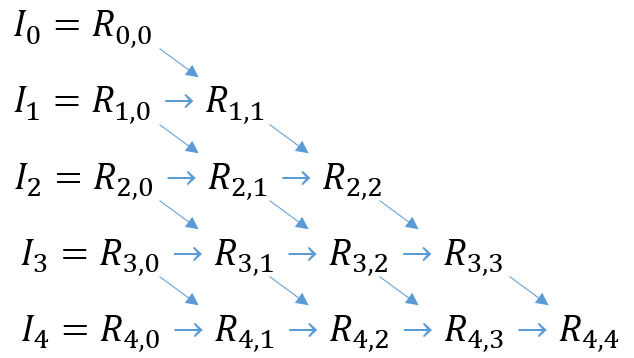
\includegraphics[width=0.5\linewidth]{fig-numint/romberg.png}}
  \caption{
  Illustration of the Romberg algorithm. Note that for each new evaluation of the integral $R_{i,0}$, all the correction terms $R_{i,m}$ (for $m>0$) must be evaluated again. \label{fig:numint:romberg}
  }
\end{figure}
%\clearpage % flush figures fig:numint:romberg


Note that the tolerance term is not the correct one as it uses the error estimate for the current step, 
which we also use correct the integral in the current step to reach a higher accuracy. 
Thus the error on the integral will always be lower than the user specified tolerance.
Below is a Python implementation:
\begin{lstlisting}[language=Python,style=blue1bar]
import numpy as np
# Function to be integrated
def f(x):
    return np.sin(x)
# step size is choosen automatically to reach (at least) 
# the specified tolerance 
def int_romberg(func, lower_limit, upper_limit,tol,show=False):
    """ calculates the area of func over the domain lower_limit
        to upper limit for the given tol, if show=True the triangular
        array of intermediate results are printed """
    Nmax = 100
    R = np.empty([Nmax,Nmax]) # storage buffer
    h = (upper_limit-lower_limit) # step size
    R[0,0]    =.5*(func(lower_limit)+func(upper_limit))*h
    N = 1
    for i in range(1,Nmax):
        h /= 2
        N *= 2
        odd_terms=0
        for all odd terms 1, 3, ..., N-1 do:
            evaulate function values at odd points,
            sum them and store in odd_terms
        R[i,0]   = 0.5*R[i-1,0] + h*odd_terms

        for all m in 0, 1, ..., i-1:
            R[i,m+1]   = R[i,m] + (R[i,m]-R[i-1,m])/(4**(m+1)-1)                  
	# check tolerance, best guess			
        calc_tol = abs(R[i,i]-R[i-1,i-1])       
        if estimated tolerance calc_tol is lower than tol:
            break  # estimated precision reached
        if max number of iterations are reached (i == Nmax-1):
            print('Romberg routine did not converge after ',
              Nmax, 'iterations!')
            
    if(show==True):
        print out all triangualar elements in R[i,m]

    return R[i,i] #return the best estimate
\end{lstlisting}

Note that the Romberg integration only uses 32 function evaluations to reach a precision of $10^{-8}$, whereas the adaptive midpoint and trapezoidal rule in the previous
section uses 20480 and 9069 function evaluations, respectively. 

\subsection{Gaussian Quadrature}
Many of the methods we have looked into are of the type:
\begin{align}
	\int_a^b f(x) dx = \sum_{k=0}^{N-1} \omega_k f(x_k),\label{eq:numint:qq1}
\end{align}
where the function is evaluated at fixed interval. For the midpoint rule $\omega_k=h$ for all values of $k$, for the trapezoid rule 
$\omega_k=h/2$ for the endpoints and $h$ for all the interior points. 
For the Simpsons rule (see exercise) $\omega_k=h/3, 4h/3,2h/3,4h/3,\ldots,4h/3,h/3$. 
Note that all the methods we have looked at so far samples the function in equal spaced points, $f(a+k h)$, 
for $k=0, 1, 2\ldots, N-1$. If we now allow for the function to be evaluated at unevenly spaced points, we can do a lot better. 
This realization is the basis for Gaussian Quadrature. We will explore this in the following, 
but to make the development easier and less cumbersome, we transform the integral from the domain $[a,b]$ to $[-1,1]$:
\begin{align}
\int_a^bf(t)dt&=\frac{b-a}{2}\int_{-1}^{1}f(x)dx\text{ , where:}\\ 
x&=\frac{2}{b-a}t-\frac{b+a}{b-a}.
\end{align}
The factor in front comes from the fact that $dt=(b-a)dx/2$, thus we can develop our algorithms on the domain $[-1,1]$, 
and then do the transformation back using: $t=(b-a)x/2+(b+a)/2$.



\begin{graybox2admon}[Notice]
The idea we will explore is as follows:
If we can approximate the function to be integrated on the domain $[-1,1]$ (or on $[a,b]$) as a 
polynomial of as \emph{large a degree as possible}, then the numerical integral of this polynomial will be very close to the integral of the 
function we are seeking.
\end{graybox2admon}



This idea is best understood by a couple of examples. Assume that we want to use $N=1$ in equation (\ref{eq:numint:qq1}):
\begin{equation}
\int_{-1}^{1}f(x)\,dx\simeq\omega_0f(x_0).
\end{equation}
We now choose $f(x)$ to be a polynomial of as large a degree as possible, but with the requirement that the integral is exact. If $f(x)=1$, we get:
\begin{equation}
\int_{-1}^{1}f(x)\,dx=\int_{-1}^{1}1\,dx=2=\omega_0,
\end{equation}
hence $\omega_0=2$. If we choose $f(x)=x$, we get:
\begin{equation}
\int_{-1}^{1}f(x)\,dx=\int_{-1}^{1}x\,dx=0=\omega_0f(x_0)=2x_0,
\end{equation}
hence $x_0=0$. 


\begin{graybox2admon}[The Gaussian integration rule for $N=1$ is:]
\begin{align}
&\int_{-1}^{1}f(x)\,dx\simeq 2f(0)\text{, or: }\nonumber\\ 
&\int_{a}^{b}f(t)\,dt\simeq\frac{b-a}{2}\,2f(\frac{b+a}{2})=(b-a)f(\frac{b+a}{2}).
\end{align}
\end{graybox2admon}



This equation is equal to the midpoint rule, by choosing $b=a+h$ we reproduce equation (\ref{eq:numint:mid0}). If we choose $N=2$:
\begin{equation}
\int_{-1}^{1}f(x)\,dx\simeq\omega_0f(x_0)+\omega_1f(x_1),
\end{equation}
we can show that now $ f(x)=1,\,x,\,x^2\,x^3$ can be integrated exact:
\begin{align}
\int_{-1}^{1}1\,dx&=2=\omega_0f(x_0)+\omega_1f(x_1)=\omega_0+\omega_1\,,\\ 
\int_{-1}^{1}x\,dx&=0=\omega_0f(x_0)+\omega_1f(x_1)=\omega_0x_0+\omega_1x_1\,,\\ 
\int_{-1}^{1}x^2\,dx&=\frac{2}{3}=\omega_0f(x_0)+\omega_1f(x_1)=\omega_0x_0^2+\omega_1x_1^2\,,\\ 
\int_{-1}^{1}x^3\,dx&=0=\omega_0f(x_0)+\omega_1f(x_1)=\omega_0x_0^3+\omega_1x_1^3\,,
\end{align}
hence there are four unknowns and four equations. The solution is: $\omega_0=\omega_1=1$ and $x_0=-x_1=1/\sqrt{3}$.


\begin{graybox2admon}[The Gaussian integration rule for $N=2$ is:]
\begin{align}
\int_{-1}^{1}f(x)\,dx&\simeq f(-\frac{1}{\sqrt{3}})+f(\frac{1}{\sqrt{3}})\, \text{, or:}\\ 
\int_{a}^{b}f(x)\,dx&\simeq \frac{b-a}{2}\left[f(-\frac{b-a}{2}\frac{1}{\sqrt{3}}+\frac{b+a}{2})
+f(\frac{b-a}{2}\frac{1}{\sqrt{3}}+\frac{b+a}{2})\right].
\end{align}
\end{graybox2admon}



\begin{lstlisting}[language=Python,style=blue1]
def int_gaussquad2(func, lower_limit, upper_limit):
    x   = np.array([-1/np.sqrt(3.),1/np.sqrt(3)])
    w   = np.array([1, 1])
    xp  = 0.5*(upper_limit-lower_limit)*x
    xp += 0.5*(upper_limit+lower_limit)
    area = np.sum(w*func(xp))
    return area*0.5*(upper_limit-lower_limit)
\end{lstlisting}

\paragraph{The case N=3.}
For the case $N=3$, we find that $f(x)=1,x,x^2,x^3,x^4,x^5$ can be integrated exactly:
\begin{align}
\int_{-1}^{1}1\,dx&=2=\omega_0+\omega_1+\omega_2\,,\\ 
\int_{-1}^{1}x\,dx&=0=\omega_0x_0+\omega_1x_1+\omega_2x_2\,,\\ 
\int_{-1}^{1}x^2\,dx&=\frac{2}{3}=\omega_0x_0^2+\omega_1x_1^2+\omega_2x_2^2\,,\\ 
\int_{-1}^{1}x^3\,dx&=0=\omega_0x_0^3+\omega_1x_1^3+\omega_2x_2^3\,,\\ 
\int_{-1}^{1}x^4\,dx&=\frac{2}{5}=\omega_0x_0^4+\omega_1x_1^4+\omega_2x_2^4\,,\\ 
\int_{-1}^{1}x^5\,dx&=0=\omega_0x_0^5+\omega_1x_1^5+\omega_2x_2^5\,,
\end{align}
the solution to these equations are $\omega_{0,1,2}=5/9, 8/9, 5/9$ and $x_{1,2,3}=-\sqrt{3/5},0,\sqrt{3/5}$. Below is a Python implementation:
\begin{lstlisting}[language=Python,style=blue1]
def int_gaussquad2(lower_limit, upper_limit,func):
    x  = np.array([-np.sqrt(3./5.),0.,np.sqrt(3./5.)])
    w  = np.array([5./9., 8./9., 5./9.])
    xp = 0.5*(upper_limit-lower_limit)*x
    xp += 0.5*(upper_limit+lower_limit)
    area = np.sum(w*func(xp))
    return area*0.5*(upper_limit-lower_limit)
\end{lstlisting}

Note that the Gaussian quadrature converges very fast. From $N=2$ to $N=3$ function evaluation we reduce the error (in this specific case) 
from 6.5\% to 0.1\%. Our standard trapezoidal formula needs more than 20 function evaluations to achieve this, the Romberg method uses 4-5 function
evaluations. How can this be? If we use the standard Taylor formula for the function to be integrated, we know that for $N=2$ the Taylor 
formula must be integrated up to $x^3$, so the error term is proportional to $h^4f^{(4)}(\xi)$ (where $\xi$ is some x-value in $[a,b]$). 
$h$ is the step size, and we can replace it with $h\sim (b-a)/N$, thus the error scale as $c_N/N^4$ (where $c_N$ is a constant). 
Following the same argument, we find for $N=3$ that the error term is $h^6f^{(6)}(\xi)$ or that the error term scale as $c_N/N^6$. 
Each time we increase $N$ by a factor of one, the error term reduces by $N^2$. Thus if we evaluate the integral for $N=10$, 
increasing to $N=11$ will reduce the error by a factor of $11^2=121$.

\subsection{Error term on Gaussian Integration}
The Gaussian integration rule of order $N$ integrates exactly a polynomial of order $2N-1$. 
From Taylors error formula, see equation (\ref{eq:taylor:error}) in Chapter~\ref{ch:taylor},
we can easily see that the error term must be of order $2N$, and be proportional to $f^{(2N)}(\eta)$, see \cite{stoer2013} for more details on the derivation of error terms. The drawback with an analytical error term derived from series expansion is that it involves the derivative of the function. As we have already explained, this is very unpractical and it is much more practical to use the methods described in section~\ref{sec:numint:parct}. Let us consider this in more detail, assume that we evaluate the integral using first a Gaussian integration rule with $N$ points, and then $N+1$ points. Our estimates of the "exact" integral, $I$,  would then be:
\begin{align}
 I&=I_N+ch_{N}^{2N},\label{eq:numint:gerr1}\\ 
 I&=I_{N+1}+ch_{N+1}^{2N+1}.
\label{eq:numint:gerr2}
\end{align}
In principle $h_{N+1}\neq h_{N}$, but in the following we will assume that $h_N\simeq h_{N+1}$, and $h\ll 1$. Subtracting equation (\ref{eq:numint:gerr1}) and (\ref{eq:numint:gerr2}) we can show that a reasonable estimate for the error term $ch^{2N}$ would be:
\begin{equation}
ch^N= I_{N+1}-I_N.
\end{equation}
If this estimate is lower than a given tolerance we can be quite confident that the higher order estimate $I_{N+1}$ approximate the true integral within our error estimate. This is the method implemented in SciPy, \href{{https://docs.scipy.org/doc/scipy-0.14.0/reference/generated/scipy.integrate.quadrature.html}}{\nolinkurl{integrate.quadrature}\footnote{\texttt{https://docs.scipy.org/doc/scipy-0.14.0/reference/generated/scipy.integrate.quadrature.html}}}
\subsection{Common Weight functions for Classical Gaussian Quadratures}
\subsection{Which method to use in a specific case?}
There are no general answers to this question, and one need to decide from case to case. If computational speed is not an issue, 
and the function to be integrated can be evaluated at any points all the methods above can be used. If the function to be integrated 
is a set of observations at different times, that might be unevenly spaced, I would use the midpoint rule:
\begin{equation}
I(a,b)=\int_a^bf(x)dx\simeq\sum_{k=0}^{N-1}M(x_k,x_k+h)=\sum_{k=0}^{N-1}h_if(x_k+\frac{h_i}{2})
\end{equation}
This is because we do not know anything about the function between the points, only when it is observed, and the formula uses only 
the information at the observation points. There is a second more subtle reason, and that is the fact that in many cases the 
observations a different times are the {\it average} value of the observable quantity and it those cases the midpoint 
rule would be the exact answer. 



% --- begin exercise ---
\begin{doconceexercise}
\refstepcounter{doconceexercisecounter}

\exercisesection{Exercise \thedoconceexercisecounter: Numerical Integration}
\addcontentsline{loe}{doconceexercise}{Exercise \thedoconceexercisecounter: Numerical Integration}



\subex{a)}
Show that for a linear function, $y=a\cdot x+b$ both the trapezoidal rule and the rectangular rule are exact

\subex{b)}
Consider $I(a,b)=\int_a^bf(x)dx$ for $f(x)=x^2$. The analytical result is $I(a,b)=\frac{b^3-a^3}{3}$. Use the Trapezoidal and 
  Midpoint rule to evaluate these integrals and show that the error for the Trapezoidal rule is exactly twice as big as the Midpoint rule.

\subex{c)}
Use the fact that the error term on the trapezoidal rule is twice as big as the midpoint rule to derive Simpsons formula: $I(a,b)=\sum_{k=0}^{N-1}I(x_k,x_k+h)=\frac{h}{6}\left[f(a)+ 4f(a+\frac{h}{2})+2f(a+h)+4f(a+3\frac{h}{2})+2f(a+2h)+\cdots+f(b)\right]$ Hint: $I(x_k,x_k+h)=M(x_k,x_k+h)+E_M$ (midpoint rule) and $I(x_k,x_k+h)=T(x_k,x_k+h)+E_T=T(x_k,x_k+h)-2E_M$ (trapezoidal rule).


% --- begin solution of exercise ---
\paragraph{Solution.}
Simpsons rule is an improvement over the midpoint and trapezoidal rule. It can be derived in different ways, we will make use of 
the results in the previous section. If we assume that the second derivative is reasonably well behaved on the interval $x_k$ 
and $x_k+h$ and fairly constant we can assume that $f^{\prime\prime}(\eta)\simeq f^{\prime\prime}(\overline{\eta})$, hence $E_T=-2E_M$.
\begin{align}
I(x_k,x_k+h)&=M(x_k,x_k+h)+E_M\text{ (midpoint rule)}\\ 
I(x_k,x_k+h)&=T(x_k,x_k+h)+E_T\nonumber\\ 
&=T(x_k,x_k+h)-2E_M\text{ (trapezoidal rule)},
\end{align}
we can now cancel out the error term by multiplying the first equation with 2 and adding the equations:
\begin{align}
3I(x_k,x_k+h)&=2M(x_k,x_k+h)+T(x_k,x_k+h)\\ 
&=2f(x_k+\frac{h}{2}) h+\left[f(x_k+h)+f(x_k)\right] \frac{h}{2}\\ 
I(x_k,x_k+h)&=\frac{h}{6}\left[f(x_k)+4f(x_k+\frac{h}{2})+f(x_k+h)\right].
\end{align}
Now we can do as we did in the case of the trapezoidal rule, sum over all the elements:
\begin{align}
I(a,b)&=\sum_{k=0}^{N-1}I(x_k,x_k+h)\nonumber\\ 
&=\frac{h}{6}\left[f(a)+ 4f(a+\frac{h}{2})+2f(a+h)+4f(a+3\frac{h}{2})\right.\nonumber\\ 
&\left.\qquad+2f(a+2h)+\cdots+f(b)\right]\\ 
&=\frac{h^\prime}{3}\left[f(a)+ f(b) + 4\sum_{k= \text{odd}}^{N-2}f(a+k h^\prime)+2\sum_{k= \text{even}}^{N-2}f(a+k h^\prime)\right],
\end{align}
note that in the last equation we have changed the step size $h=2h^\prime$.

% --- end solution of exercise ---

\subex{d)}
Show that for $N=2$ ($f(x)=1,x,x^3$), the points and Gaussian quadrature rule for $\int_{0}^{1}x^{1/2}f(x)\,dx$
is $\omega_{0,1}=-\sqrt{70}{150} + 1/3, \sqrt{70}{150} + 1/3$
and $x_{0,1}=-2\sqrt{70}{63} + 5/9, 2\sqrt{70}{63} + 5/9$
\begin{enumerate}
\item Integrate $\int_0^1x^{1/2}\cos x\,dx$ using the rule derived in the exercise above and compare with the standard Gaussian quadrature rule for ($N=2$, and $N=3$).
\end{enumerate}

\noindent
\subex{e)}
Make a Python program that uses the Midpoint rule to integrate experimental data that are unevenly spaced and given in the form of two arrays.




\end{doconceexercise}
% --- end exercise ---


% !split
\chapter{Ordinary differential equations}
\label{ch:ode}
% !split
\chapter{Monte Carlo Methods}
\label{ch:mc}

% !split

\clearemptydoublepage
\markboth{Bibliography}{Bibliography}
\thispagestyle{empty}

\bibliographystyle{plain}
\bibliography{../chapters/papers}

% ------------------- end of main content ---------------

% #ifdef PREAMBLE
\end{document}
% #endif

